\chapter{Architectural Implications of Sparse Tensor Workloads} \label{sec:architectural-implications}

This chapter derives the architectural requirements that motivate the TMU--CPU system developed in the rest of the thesis. We study two complementary classes of sparse tensor workloads. Scientific sparse tensor kernels expose the diversity of sparse tensor algebra: they combine sparse traversal, scan-and-lookup operations, coordinate merging, and computation on partial results. These workloads show that general-purpose processors already provide several capabilities that sparse tensor algebra needs, including large memory capacity, caches that can exploit locality, vector units for dense arithmetic, and flexible general-purpose execution. However, they are inefficient at the irregular traversal, merging, and lookup operations that account for most execution cycles of these workloads. Machine learning embedding workloads isolate the most important of these bottlenecks: irregular lookup and accumulation of dense embedding vectors. Although these workloads are less diverse in their sparse operations, they expose a wide range of spatial and temporal locality because they access vectors of different sizes with different reuse patterns. This makes them useful for quantifying how locality affects cache filtering, memory-level parallelism, and request-tracking requirements. Together, these two studies show that traditional architectures, which execute traversal, merging, lookup, and computation on the same compute cores, cannot scale efficiently to the requirements of sparse tensor algebra. They motivate decoupling sparse traversal and merging from computation, which is the design principle implemented by the TMU.

\section{Sparse Scientific Computing} \label{sec:sparse-scientific-computing} %%%%%%%%%%%%%%%%%%%%%%%%%%%%%%%

Scientific sparse kernels provide the broadest view of the architectural requirements of sparse tensor algebra. They exercise the main sparse operations discussed in \Cref{sec:sparse-tensor-algebra-fundamentals}: traversal to recover compressed coordinates and values, scan-and-lookup to access dense or sparse operands indirectly, merging to co-iterate sparse operands, and computation over the resulting partial results. This makes them a useful starting point for separating what general-purpose processors already do well from what they handle inefficiently.

\subsection{Scientific Workload Methodology} \label{sec:scientific-workload-methodology} %%%%%%%%%%%%%%%%%%%%%%%%%%%%%%%%%%%%%%%%%%%%%%%%%%%%%%%%%%%%%%%%%%%%%

To broadly understand the architectural implications of sparsity, we study three representative kernels across a large and diverse set of inputs on two processors with very different architectural characteristics.

We analyze the three main kernels introduced in \Cref{sec:sparsity-in-scientific-computing}, each chosen to isolate a distinct architectural stressor:
\begin{itemize}
    \item \emph{Sparse Matrix--Vector Multiplication} (SpMV)~\cite{williams2007sc}, which multiplies a CSR matrix and a dense vector and outputs a dense vector ($Z_i = A_{ij} B_j$). Since co-iteration of $A_{*j}$ and $B_j$ is generally implemented as a memory-intensive scan-and-lookup operation (\Cref{sec:scan-and-lookup}), we use SpMV as a proxy for sparse traversal and indirect scalar lookup.
    \item \emph{Gustavson's Sparse Matrix--Sparse Matrix Multiplication} (SpMSpM)~\cite{gao2023systematic}, which multiplies and outputs CSR matrices ($Z_{ij} = A_{ik} B_{kj}$ with $(ikj)$ schedule). SpMSpM performs the same scan-and-lookup operation as SpMV but, instead of scalars, it looks up and loads whole (sparse) rows of $B$, which are then reduced into a single row. For this reason, SpMSpM is a proxy for scan-and-lookup operations with higher spatial locality, as well as for the accumulation of intermediate results.
    \item \emph{Sparse Matrix Addition} (SpAdd)~\cite{hussain2022ipdps}, which adds and outputs CSR matrices ($Z_{ij} = A_{ij} + B_{ij}$) by repeatedly co-iterating and joining (disjunctive merge) matrix fibers with the same row index $i$. Therefore, SpAdd is representative of coordinate merging and the data-dependent control flow it induces.
\end{itemize}

We profile high-performance implementations of these kernels from Kokkos version 3.5~\cite{edwards2014kokkos} on both an HPC processor, the Fujitsu A64FX~\cite{sato2020design}, and a data-center processor, the AWS Graviton~3~\cite{aws2026graviton,aws2022c7g}. The main architectural characteristics of the two processors are summarized in \Cref{tab:implications-scientific-cpu-specs}. While the two processors provide similar peak compute throughput, the A64FX provides more than 3$\times$ the memory bandwidth, whereas the Graviton~3 provides more cores and more aggressive out-of-order resources. To capture widely different input features, we test these kernels on 1000 of the largest SuiteSparse matrices, spanning diverse application domains~\cite{davis2011university}.

\begin{table}
    \centering
    \footnotesize
    \caption[Specifications of the CPUs used for sparse scientific workloads.]{Specifications of the CPUs used for the sparse scientific workload characterization~\cite{sgherzi2024jpdc,sato2020design,aws2026graviton}.}
    \vspace{-0.5em}
    \begin{tabular}{p{0.22\linewidth}p{0.32\linewidth}p{0.32\linewidth}}
        \toprule
        & \textbf{A64FX} & \textbf{Graviton~3} \\
        \midrule
        Manufacturer & Fujitsu & Amazon \\
        Architecture & ARM v8.2 & ARM v8.4 \\
        Core type & Fujitsu superscalar OoO HPC core & Arm Neoverse-V1 OoO server core \\
        Design target & Dense scientificg computation & General-purpose server workloads \\
        Sockets & 1 & 1 \\
        Cores per socket & 48 & 64 \\
        Vector units & 2 $\times$ 512-bit SVE & 2 $\times$ 256-bit SVE \\
        Peak FP64 performance & 3.38 TFLOP/s & 2.66 TFLOP/s \\
        L1D, L1I per core & 64 kB, 64 kB & 64 kB, 64 kB \\
        Private L2 & N/A & 64 $\times$ 1 MB \\
        Shared LLC & 4 $\times$ 8 MB & 32 MB \\
        Memory technology & HBM2 & DDR5 \\
        Memory channels & 32 & 8 \\
        Peak bandwidth & 1024 GB/s & 300 GB/s \\
        Operating System & Red Hat Enterprise Linux 8.1 & Ubuntu 22.04 \\
        Compiler & armclang 22.0.2 & armclang 22.0.2 \\
        \bottomrule
    \end{tabular}
    \label{tab:implications-scientific-cpu-specs}
\end{table}

\subsection{CPU Performance Characterization} \label{sec:scientific-cpu-performance-characterization} %%%%%%%%%%%%%%%%%%%%%%%%%%%%%%%%%%%%%%%%%%%%%%%%%%%%%%%%%%%%%%%%%%%%%

In this section, we show that neither off-the-shelf HPC processors nor data-center processors efficiently handle the irregular operations that dominate sparse scientific workloads. Although these designs provide different balances of memory bandwidth, vector throughput, cache capacity, and out-of-order execution resources, sparse traversal and merging still leave substantial compute and memory resources underutilized.

\begin{figure}
     \centering
     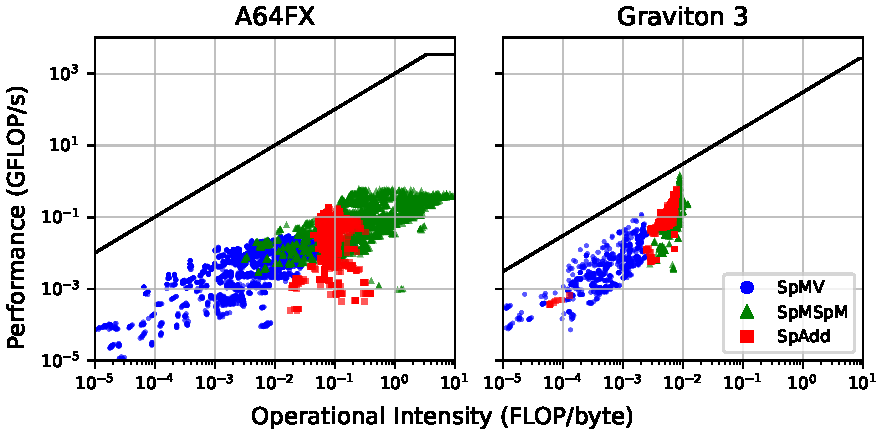
\includegraphics[width=0.7\columnwidth]{img_roofline_numeric.pdf}
     \caption[Roofline model of scientific kernels on CPU.]{Roofline model of sparse scientific kernels on 1000 of the largest SuiteSparse matrices, spanning diverse application domains, evaluated with Kokkos on A64FX (left) and Graviton~3 (right). The black lines are the processor-specific Roofline ceilings from peak compute throughput and peak memory bandwidth. The x-axis reports operational intensity, computed as floating-point operations per byte transferred from main memory by the measured execution (FLOP/byte), and the y-axis reports achieved performance (GFLOP/s); both axes use logarithmic scales. For sparse kernels, the byte count includes accesses to compressed-format metadata, nonzero values, dense operands, intermediate data structures, and output data. Each point is one matrix; blue, green, and red points correspond to SpMV, SpMSpM, and SpAdd, respectively. Overall, performance increases with operational intensity across kernels and inputs. However, despite achieving higher cache utilization, the A64FX does not consistently outperform the Graviton~3.}
     \label{fig:implications-scientific-roofline}
\end{figure}


\begin{table}[htbp!]
\centering
\footnotesize
\caption[Summary of CPU resource utilization for sparse scientific kernels.]{Minimum, average, and maximum resource utilization for the sparse scientific kernels. Values are percentages of each processor's peak compute throughput and peak memory bandwidth. Each subtable reports one kernel, rows correspond to A64FX and Graviton~3, and columns summarize the distribution across 1000 of the largest SuiteSparse matrices, spanning diverse application domains. Compute utilization is extremely low for all kernels: the maximum is 1.8e-2\% on A64FX and 5.7e-2\% on Graviton~3, both for SpMSpM. Bandwidth utilization is higher and more variable: averages range from 0.046\%--0.28\% on A64FX and 2.3\%--9.8\% on Graviton~3, with maxima of 1.7\% and 56\%, respectively. Thus, sparse scientific kernels use little of the available compute throughput, while memory-bandwidth utilization depends strongly on both architecture and input matrix.}
\label{tab:utilization}

%==================== SpMV ====================
\begin{subtable}{\linewidth}
\centering
\caption{SpMV}
\begin{tabular}{c|ccc|ccc}
\toprule
& \multicolumn{3}{c|}{\textbf{Compute}} & \multicolumn{3}{c}{\textbf{Bandwidth}} \\
& Min & Avg & Max & Min & Avg & Max \\
\midrule

\textbf{A64FX} & 3.2e-7 & 9.0e-5 & 9.5e-4 & 1.2e-3 & 2.8e-1 & 1.7 \\
\textbf{Graviton~3} & 1.1e-6 & 2.5e-4 & 4.6e-3 & 1.8e-1 & 2.3 & 2.1e1 \\

\bottomrule
\end{tabular}
\end{subtable}

\vspace{0.5em}

%==================== SpMSpM ====================
\begin{subtable}{\linewidth}
\centering
\caption{SpMSpM}
\begin{tabular}{c|ccc|ccc}
\toprule
& \multicolumn{3}{c|}{\textbf{Compute}} & \multicolumn{3}{c}{\textbf{Bandwidth}} \\
& Min & Avg & Max & Min & Avg & Max \\
\midrule

\textbf{A64FX} & 2.9e-5 & 4.9e-3 & 1.8e-2 & 7.4e-5 & 7.5e-2 & 4.0e-1 \\
\textbf{Graviton~3} & 2.4e-10 & 9.8e-3 & 5.7e-2 & 2.1e-2 & 9.8 & 5.6e1 \\

\bottomrule
\end{tabular}
\end{subtable}

\vspace{0.5em}

%==================== SpAdd ====================
\begin{subtable}{\linewidth}
\centering
\caption{SpAdd}
\begin{tabular}{c|ccc|ccc}
\toprule
& \multicolumn{3}{c|}{\textbf{Compute}} & \multicolumn{3}{c}{\textbf{Bandwidth}} \\
& Min & Avg & Max & Min & Avg & Max \\
\midrule

\textbf{A64FX} & 5.9e-9 & 1.5e-3 & 5.3e-3 & 1.4e-4 & 4.6e-2 & 2.2e-1 \\
\textbf{Graviton~3} & 5.0e-8 & 4.5e-3 & 2.2e-2 & 5.8e-1 & 5.8 & 2.5e1 \\

\bottomrule
\end{tabular}
\end{subtable}

\end{table}


\Cref{fig:implications-scientific-roofline} presents the Roofline models of these kernels and matrices on the two evaluated processors. Overall, all kernels and matrices are heavily memory bound on both processors, and performance generally increases with operational intensity. For both processors, SpMV has the lowest operational intensity and performance across kernels, whereas SpMSpM has the highest due to partial-result accumulation, and SpAdd falls between the two. Across processors, the A64FX makes better use of caches and achieves higher operational intensity for all kernels, but it does not necessarily achieve higher performance than the Graviton~3.

\begin{figure}
     \centering
     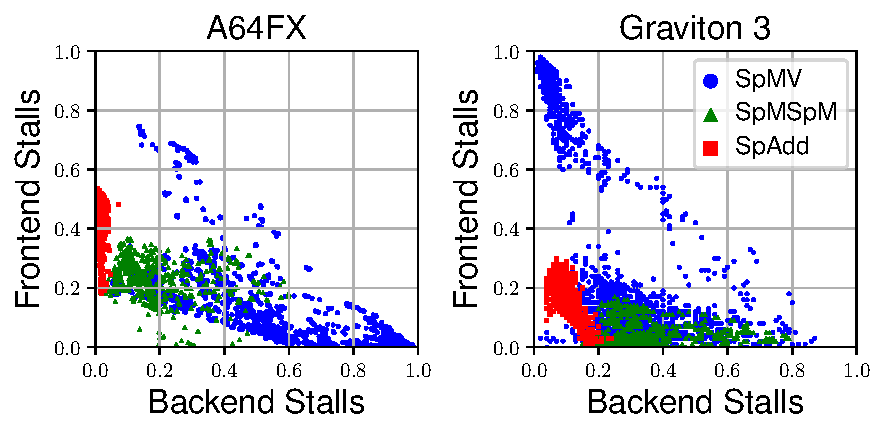
\includegraphics[width=0.7\columnwidth]{img_backend_vs_frontend.pdf}
     \caption[Cycles spent stalling in scientific kernels on CPU.]{Frontend and backend stalls for the sparse scientific kernels on 1000 of the largest SuiteSparse matrices, spanning diverse application domains, evaluated with Kokkos on A64FX (left) and Graviton~3 (right). Stall cycles are normalized to total execution cycles. The x-axis reports the fraction of cycles with backend stalls, which capture delays in compute units and the memory hierarchy, and the y-axis reports the fraction of cycles with frontend stalls, which capture instruction-pipeline inefficiencies such as branch mispredictions. These two quantities are measured independently and are not mutually exclusive: a cycle may contain both frontend and backend stalls, so the two fractions need not sum to one. Each point is one matrix; blue, green, and red points correspond to SpMV, SpMSpM, and SpAdd, respectively. Overall, both data-dependent control and irregular memory accesses generate large stall fractions, limiting performance.}
     \label{fig:implications-scientific-stalls}
\end{figure}

\begin{table}[htbp!]
\centering
\footnotesize
\caption[Summary of stall cycles for different processors and kernels.]
{Minimum, average, and maximum frontend and backend stalls on A64FX and Graviton 3 for SpMV, SpMSpM, SpAdd.}
\label{tab:stalls}

\begin{tabular}{cc|rrr|rrr|rrr}
\toprule
& &
\multicolumn{3}{c|}{\textbf{SpMV}} &
\multicolumn{3}{c|}{\textbf{SpMSpM}} &
\multicolumn{3}{c}{\textbf{SpAdd}} \\
& &
\textbf{Min} & \textbf{Avg} & \textbf{Max} &
\textbf{Min} & \textbf{Avg} & \textbf{Max} &
\textbf{Min} & \textbf{Avg} & \textbf{Max} \\
\midrule

\multirow{2}{*}{\textbf{A64FX}}
& \textbf{Frontend stalls}
& 0\% & 33\% & 78\%
& 0\% & 28\% & 37\%
& 16\% & 42\% & 54\% \\

& \textbf{Backend stalls}
& 2\% & 63\% & 99\%
& 3\% & 21\% & 61\%
& 0\% & 6\% & 8\% \\

\midrule

\multirow{2}{*}{\textbf{Graviton 3}}
& \textbf{Frontend stalls}
& 0\% & 58\% & 98\%
& 0\% & 7\% & 18\%
& 0\% & 21\% & 29\% \\

& \textbf{Backend stalls}
& 1\% & 28\% & 86\%
& 14\% & 38\% & 79\%
& 4\% & 14\% & 26\% \\

\bottomrule
\end{tabular}
\end{table}


To better understand the reason, we measure the fraction of frontend and backend stalls on each processor, reported in \Cref{fig:implications-scientific-stalls} and summarized in \Cref{tab:implications-scientific-stall-summary}. Frontend stalls arise from inefficiencies in the instruction pipeline, whereas backend stalls originate from inefficiencies in the compute units and memory subsystem. For sparse kernels, frontend stalls are primarily caused by branch mispredictions in data-dependent loop branches. Backend stalls are largely due to irregular memory accesses, which generate long-latency memory operations that block the compute pipeline~\cite{dongarra2013metric,dongarra2013hpcg,talati2021hpca,talati2022isca}. This leads to three observations:
\begin{itemize}
    \item For SpMV, unlike the Graviton~3, the A64FX exhibits substantially more backend stalls than frontend stalls (63\% vs. 33\% on average). We attribute this behavior to the A64FX being primarily optimized for regular high-throughput computation and therefore being less resilient to irregular memory accesses. Its relatively small cores provide limited instruction-level and memory-level parallelism for tolerating long memory latencies~\cite{esmailidokht2024micro}. In contrast, the Graviton~3 exhibits a larger fraction of frontend stalls (58\% frontend vs. 28\% backend on average), likely because its more aggressive cores sustain higher memory-level parallelism while incurring higher branch misprediction penalties.
    
    \item For SpMSpM, the A64FX achieves better backend utilization than in SpMV, with average backend stalls falling from 63\% to 21\%. Conversely, on the Graviton~3, SpMSpM exhibits backend utilization comparable to SpMV, with average backend stalls of 38\% and 28\%, respectively. These results suggest that (i)~scan-and-lookup operations with higher spatial locality benefit significantly from high-bandwidth architectures, and (ii)~reduction operations do not severely impact backend utilization because partial results typically fit in cache~\cite{nagasaka2018high}. However, computing these reductions benefits from stronger frontend capabilities and more aggressive speculation, such as those provided by the Graviton~3 cores.
    
    \item For SpAdd, the frontend becomes the dominant bottleneck due to highly data-dependent branching behavior, particularly on cores with limited out-of-order execution capabilities such as those in the A64FX, where average frontend stalls reach 42\% compared with only 6\% backend stalls~\cite{hussain2022ipdps}.
\end{itemize}

In conclusion, our study suggests that off-the-shelf CPU cores are not optimized for the irregular control flow and memory operations characteristic of sparse scientific workloads. Data-dependent control flow triggers branch mispredictions that stall the frontend, while irregular memory operations create long-latency fetches that stall the backend. Caches can reduce this cost when locality is available, but they are not sufficient to eliminate the bottleneck. In the next section, we use machine learning workloads---with their wider range of spatial and temporal locality characteristics---to study this limitation further.

\section{Machine Learning Embedding Workloads} \label{sec:ml-embedding-workloads} %%%%%%%%%%%%%%%%%%%%%%%%%%%%%%%

The scientific kernels show that sparse tensor algebra stresses processors through a combination of traversal, scan-and-lookup, merging, and computation. Machine learning embedding workloads let us study the most important of these stressors in isolation: irregular lookup and accumulation of dense embedding vectors. This narrower structure is useful because embedding operations access fixed-size vectors, making spatial locality explicit, and because different models and inputs reuse those vectors at very different rates, making temporal locality explicit. We therefore use embedding workloads to quantify how spatial and temporal locality shape cache behavior, memory-level parallelism, and the request-tracking resources required by conventional architectures. We first characterize these workloads to identify their compute, memory-capacity, and locality requirements. We then show that GPUs, despite being the de facto architecture for machine learning, are inadequate for embedding operations because irregular lookups underutilize their bandwidth and compute resources. Next, we discuss the cost potential of CPUs for these workloads, but show that commodity cores achieve low performance because they cannot sustain enough irregular memory requests. Finally, we build an analytical model to show that this limitation cannot be solved by simply scaling conventional core resources.

\subsection{Embedding Workload Methodology} \label{sec:embedding-workload-methodology} %%%%%%%%%%%%%%%%%%%%%%%%%%%%%%%%%%%%%%%%%%%%%%%%%%%%%%%%%%%%%%%%%%%%%

Our GPU measurements use an NVIDIA H100 GPU. We measure GPU performance with NVIDIA Nsys~\cite{nvidia2024nsys} and report only device kernel execution time, excluding host-to-device transfers.

\begin{table}[]
    \centering
    %\footnotesize
    \caption[Specifications of the multicore CPU processor used in our study (baseline).]{Specifications of the multicore CPU processor used in our study, a beefy HPC processor with Arm-like cores, HBM, and large caches.}
    \vspace{-0.5em}
    \begin{tabular}{rl}
        \toprule
        SiP & 96 cores \& LLC slices, 6 HBM stacks. \\
        Core & N1-like OoO core @ 2.4\,GHz, 224-entry ROB, 2$\times$96-entry LSQ. \\
        Comp & 2$\times$64B vector units per core, one 64B$\times$64B matrix unit per core. \\
        L1D & 64\,KiB/core, 4-way, 2-cycle access, 32 MSHRs, stride/IMP prefetcher. \\
        L2 & 512\,KiB/core, 8-way, 8-cycle access, 64 MSHRs, best-offset prefetcher. \\
        LLC & Mostly exclusive, 1\,MiB/slice, 16-way, 12-cycle access, 128 MSHRs. \\
        NoC & 2D mesh, 1-cycle routers, 1-cycle links, MOESI-like AMBA~5 CHI. \\
        HBM & HBM3, 560\,GB/s per stack, 12\,GB per stack. \\
        %TMU & 8\,KiB storage, 256 MSHRs, 1\,GHz. \\        
        \bottomrule
    \end{tabular}
    \label{tab:cpu-specs-embedding}
\end{table}

To estimate how conventional CPU architectures scale on embedding operations, unlike the previous section, we use gem5~\cite{lowepower2020gem5} for CPU performance estimation and McPAT~\cite{li2009micro} for power estimation. This simulation-based methodology allows us to vary critical microarchitectural resources such as the reorder buffer (ROB), load-store queue (LSQ), and miss status holding registers (MSHRs), which cannot be controlled on fixed commercial processors. The baseline CPU system, dimensioned as in \Cref{tab:embedding-cpu-system-specs}, models a datacenter-class multicore processor with HBM, HBM bandwidth comparable to the Nvidia H100 GPU~\cite{nvidia2024h100}, and bandwidth per core and per-core performance in the range of commercial HBM-based CPUs~\cite{reguly2023xeonmax}.

\begin{table}
  \centering
  \caption[Tested Deep Learning Recommendation Model configurations.]{Deep Learning Recommendation Model (DLRM) embedding configurations evaluated in this chapter. RM1, RM2, and RM3 vary the number of segments per batch per core, embedding-vector length, and lookups per segment. Larger batches amortize per-batch startup overhead, longer embedding vectors increase spatial locality but also increase cache pressure, and more lookups per segment amortize per-segment loop-control overhead.}
  \vspace{-1em}
\[
\begin{tabular}{rccc}
\toprule
  \textbf{Property Description} & \textbf{RM1} & \textbf{RM2} & \textbf{RM3} \\
\toprule
  \textbf{Segments per batch per core} & 64 & 32 & 16 \\
  \textbf{Elements per embedding vector} & 32 & 64 & 128 \\
  \textbf{Lookups per segment} & 64 & 128 & 256 \\
\hline
\end{tabular}
\]
  \label{tab:embedding-dlrm-configurations}
\end{table}

\begin{table}
  \centering
  %\footnotesize
  \caption[Selected inputs for graph-learning models.]{Typical inputs for graph-learning models. Layer sizes indicate the size of the embedding vectors, defined as the number of elements. For GNNs, we report the embedding size of each layer.}
  \vspace{-1em}
\[
\begin{tabular}{cccccc}
\toprule
  \textbf{Model} & \textbf{Input} & \textbf{\#Nodes} & \textbf{\#Edges} & \textbf{Layers sizes} \\
\toprule
  GNN & \texttt{arxiv}~\cite{ogb2020neurips} & 0.2M & 1.2M & 128$\times$256$\times$256$\times$40 \\
  GNN & \texttt{mag}~\cite{ogb2020neurips} & 1.9M & 21.1M & 128$\times$256$\times$349 \\
  GNN & \texttt{products}~\cite{ogb2020neurips} & 2.4M & 61.9M & 100$\times$256$\times$256$\times$47 \\
  GNN & \texttt{proteins}~\cite{ogb2020neurips} & 0.1M & 39.6M & 8$\times$256$\times$256$\times$112\\
\hline
  MP & \texttt{com-Youtube}~\cite{snapnets2014} & 1.1M & 6.0M & 128 \\
  MP & \texttt{roadNet-CA}~\cite{snapnets2014} & 2.0M & 5.5M & 128 \\
  MP & \texttt{web-Google}~\cite{snapnets2014} & 0.9M & 5.1M & 128 \\
  MP & \texttt{wiki-Talk}~\cite{snapnets2014} & 2.4M & 5.0M & 128 \\
\hline
  KG & \texttt{biokg}~\cite{ogb2020neurips} & 0.1M & 5.1M & 512 \\
  KG & \texttt{wikikg2}~\cite{ogb2020neurips} & 2.5M & 17.1M & 512 \\
\bottomrule
\end{tabular}
\]
  \label{tab:graph-inputs}
  %\vspace{-2em}
\end{table}


All embedding operations we test are high-performance multicore implementations from the literature. For DLRMs, we use state-of-the-art EB implementations such as those in PyTorch~\cite{paszke2019neurips} and Glow~\cite{smelyanskiy2018arxiv}, and test the three configurations in \Cref{tab:embedding-dlrm-configurations}, each with low- (\texttt{L0}), medium- (\texttt{L1}), and high-locality (\texttt{L2}) inputs~\cite{gupta2020hpca,gupta2020isca}. For LLMs, we test the original BigBird code and settings~\cite{zaheer2020neurips} while varying the block size. For GNNs and KGs, we use the OGB~\cite{hu2020neurips} PyTorch implementations, whereas for MP we adapt the code from FusedMM~\cite{rahman2021ipdps}. For these graph-learning models, we use the inputs and feature sizes reported in \Cref{tab:embedding-graph-inputs}, drawn from OGB~\cite{hu2020neurips} or Snap/SuiteSparse~\cite{leskovec2014snap,davis2011university}.

\subsection{Embedding Workload Characterization} \label{sec:embedding-workload-characterization} %%%%%%%%%%%%%%%%%%%%%%%%%%%%%%%%%%%%%%%%%%%%%

\begin{table}[]
    \centering
    \caption[Algorithmic characterization of embedding operations.]{Algorithmic characterization of the embedding operations studied in \Cref{sec:embedding-workload-characterization}. The table summarizes each operation's loop hierarchy and its compute-per-lookup ratio, using one dense embedding-vector lookup as the normalization baseline. The ratio counts vector arithmetic operations performed for each irregular vector lookup. EB performs one vector accumulation per lookup, KGs perform four vector operations across three lookups, SpMM performs one rescale and one accumulation per lookup, and MP reaches the highest ratio with at most five vector operations across two lookups. SpAttn performs no arithmetic on the looked-up vectors in this characterization because it copies sparse-attention blocks. Thus, the compute-per-lookup ratio ranges from 0 to at most 2.5, showing that these embedding operations expose little arithmetic work per irregular lookup and therefore give compute-oriented architectures limited opportunity to hide lookup latency.}
    \begin{tabular}{clc}
        \toprule
            \makecell[c]{\textbf{Op}} & 
            \makecell[l]{\textbf{Loop hierarchy}} & 
            $\frac{\textbf{N}_\textbf{compute}}{\textbf{N}_\textbf{lookups}}$\\
        \toprule
            \makecell[c]{SpMM \\(GNNs)} &% \\ (\Cref{sec:embedding-characterization-graph-learning})} &
            \makecell[l]{$\forall$ vertex in graph\\
                        \hspace{0.5em}$\forall$ neighbor of vertex\\
                            \hspace{1em}\textbf{lookup} vector\\
                            \hspace{1em}\textbf{rescale} vector\\
                            \hspace{1em}\textbf{accumulate} vector} &
            $\frac{2}{1}$\\
        \hline
            \makecell[c]{MP} &% \\ (\Cref{sec:embedding-characterization-graph-learning})} &
            \makecell[l]{$\forall$ vertex in graph\\
                        \hspace{0.5em}\textbf{lookup} vertex vector\\
                        \hspace{0.5em}$\forall$ neighbor of vertex\\
                            \hspace{1em}\textbf{lookup} neighbor vector\\
                            \hspace{1em}\textbf{multiply} vert-neigh vecs\\
                            \hspace{1em}\textbf{scale} and \textbf{accumulate} vec\\
                        \hspace{0.5em}\textbf{multiply-accumulate} vec} &
            $\leq\frac{5}{2}$\\
        \hline
            \makecell[c]{KGs} &% \\ (\Cref{sec:embedding-characterization-graph-learning})} &
            \makecell[l]{$\forall$ sample in batch\\
                            \hspace{0.5em}\textbf{lookup} vector\\
                            \hspace{0.5em}\textbf{compute} h-r-l norm} &
            $\frac{4}{3}$\\
        \hline
            \makecell[c]{EB \\ (DLRMs)} &% \\ (\Cref{sec:embedding-characterization-dlrms})} &
            \makecell[l]{$\forall$ segment in batch\\
                            \hspace{0.5em}$\forall$ category in segment\\
                                \hspace{1.0em}\textbf{lookup} vector\\
                                \hspace{1.0em}\textbf{accumulate} vector} &
            $\frac{1}{1}$\\
        \hline
            \makecell[c]{SpAttn \\ (LLMs)} &% \\ (\Cref{sec:embedding-characterization-llms})} &
            \makecell[l]{$\forall$ block in Q input\\
                        \hspace{0.5em}$\forall$ block in K input\\
                            \hspace{1.0em}$\forall$ token in K block\\
                                \hspace{1.5em}\textbf{lookup} K vector\\
                                \hspace{1.5em}$\forall$ token in Q block\\
                                    \hspace{2em}\textbf{copy} K vector} &
            $0$\\
        \bottomrule
    \end{tabular}
    \label{tab:embedding-workload-code-characterization}
\end{table}

\begin{table}[]
    \centering
    \caption[Memory characterization of embedding operations.]{Memory characterization of the embedding operations studied in \Cref{sec:embedding-workload-characterization}. The table reports embedding storage requirements, temporal locality, and spatial locality. Temporal locality is measured with the reuse-distance CDF: the x-axis is cache capacity measured in embedding vectors, and the y-axis is the fraction of accesses whose reuse distance is below that capacity. Thus, the y-value approximates the hit probability of a cache that can hold the corresponding number of embedding vectors. Spatial locality is measured by the number of elements fetched per embedding-vector lookup. Temporal locality varies widely across workloads and inputs. At a reuse distance of 1K vectors, GNN CDFs stay below 20\%---meaning that fewer than 20\% of accesses have reuse distance below 1K vectors---and KGs below 10\%, while MP ranges from below 5\% to roughly 45\% depending on the input graph. DLRMs exhibit higher but feature-dependent locality, with Criteo features reaching about 63\%--99\% CDF at 1K vectors. Sparse attention locality depends strongly on block size: larger blocks increase the CDF but also increase copied-vector work. Spatial locality also varies widely, from 8--349 elements for GNNs, 128 for MP, 512 for KGs, 32--256 for EB, and up to $8\times8\times512$ elements for sparse attention blocks. Together, these ranges show that embedding workloads need architectures that adapt to widely different temporal and spatial locality regimes, exploiting cache reuse when it exists while also sustaining low-reuse vector lookups with different vector sizes.}
    \begin{tabular}{ccccc}
        \toprule
            \makecell[c]{\textbf{Op}} & 
            \makecell[c]{\textbf{Memory} \\ \textbf{footprint}} &
            \makecell[c]{\textbf{Temporal locality} \\ \textbf{(reuse distance CDF)}} &
            \makecell[c]{\textbf{Spatial locality} \\ \textbf{(vector dim.)}}\\
        \toprule
            \makecell[c]{SpMM \\(GNNs)} &% \\ (\Cref{sec:embedding-characterization-graph-learning})} &
            \makecell{Single embedding \\ table GBs large} &
            \vcentered{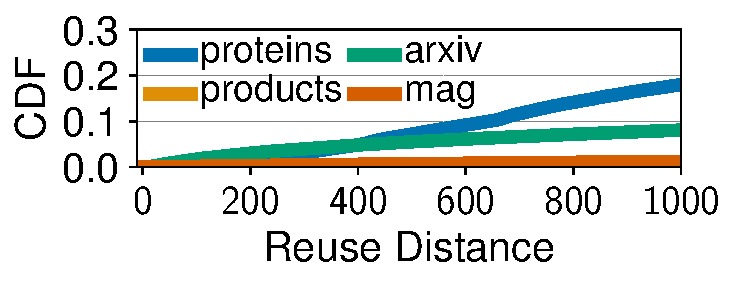
\includegraphics[width=.35\linewidth]{img_cdf_gnn.pdf}} &
            8-349\\ 
        \hline
            \makecell[c]{MP} &% \\ (\Cref{sec:embedding-characterization-graph-learning})} &
            \makecell{Two embedding tables, \\ each GBs large} &
            \vcentered{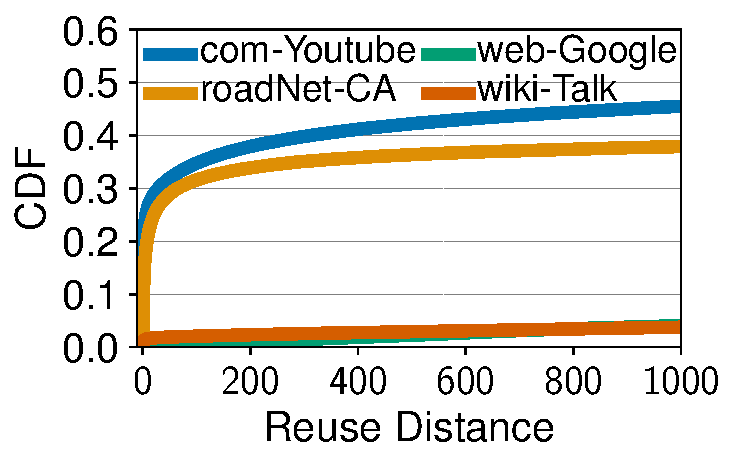
\includegraphics[width=.35\linewidth]{img_cdf_mp.pdf}} &
            128\\
        \hline
            \makecell[c]{KGs} &% \\ (\Cref{sec:embedding-characterization-graph-learning})} &
            \makecell{Single embedding \\ table GBs large} &
            \vcentered{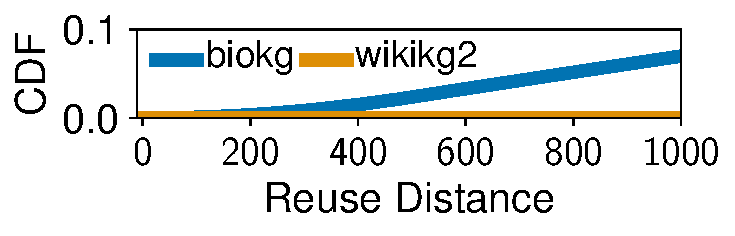
\includegraphics[width=.35\linewidth]{img_cdf_kg.pdf}} &
            512\\
        \hline
            \makecell[c]{EB \\ (DLRMs)} &% \\ (\Cref{sec:embedding-characterization-dlrms})} &
            \makecell{All embedding tables \\ require GBs~\cite{gupta2020hpca}\\ to TBs~\cite{ibrahim2022memsys}} &
            \vcentered{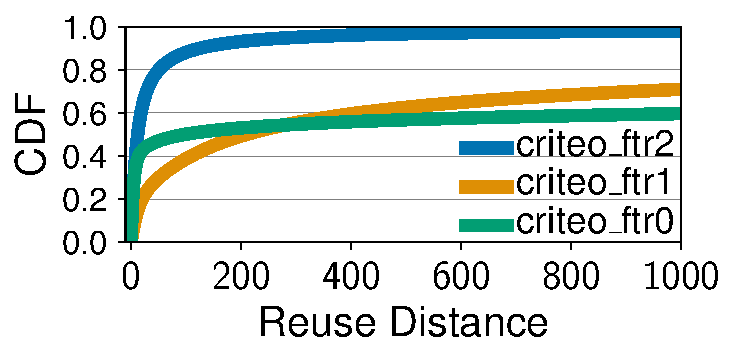
\includegraphics[width=.35\linewidth]{img_cdf_dlrm.pdf}} &
            32-256\\
        \hline
            \makecell[c]{SpAttn \\ (LLMs)} &% \\ (\Cref{sec:embedding-characterization-llms})} &
            \makecell{K-V tensors are MBs \\ Out tensor is MB-GB} &
            \vcentered{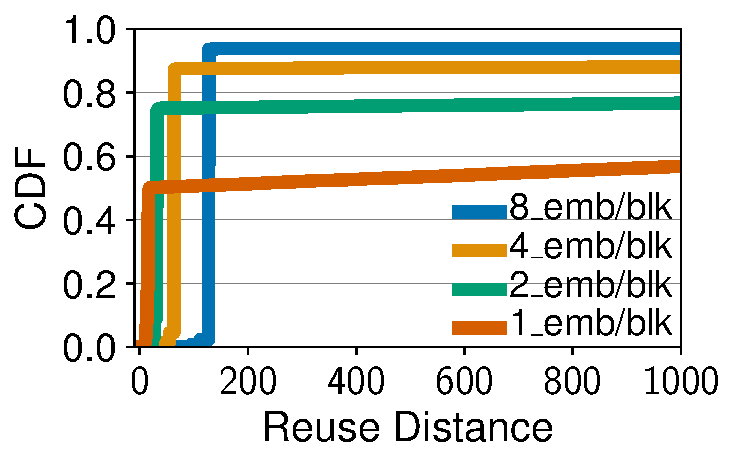
\includegraphics[width=.35\linewidth]{img_cdf_llm.pdf}} &
            $\leq$ 8x8x512\\
        \bottomrule
    \end{tabular}
    \label{tab:embedding-workload-locality-characterization}
\end{table}


Before evaluating traditional architectures, we first characterize the properties that determine how embedding operations interact with the memory hierarchy. In particular, we study their loop structure, compute-per-lookup ratio, memory footprint, temporal locality, and embedding-vector size, which together determine whether caches, prefetching, memory bandwidth, or core-side request tracking are likely to become the bottleneck.

\Cref{tab:embedding-workload-code-characterization} characterizes the code structure of embedding operations across several machine learning models, whereas \Cref{tab:embedding-workload-locality-characterization} characterizes their memory requirements. For each model, we first analyze its loop hierarchy and compute-per-lookup ratio, which approximate compute requirements. We then compute the memory footprint of the embedding tables to understand their storage demands. Finally, we characterize temporal locality with reuse-distance CDFs and spatial locality with embedding-vector sizes to gauge the effectiveness of caches and prefetchers for embedding lookups.

We characterize temporal locality through the concept of \emph{reuse distance}---the number of other vectors accessed before a vector is accessed again~\cite{ding2003pldi}. If a cache can hold $x$ vectors, an access with reuse distance greater than $x$ will likely result in eviction. For a given input, we first construct a histogram of all reuse distances, which we then integrate and normalize to obtain the cumulative distribution function (CDF). Hence, $CDF(x)$ approximates the hit probability for a cache that can hold $x$ vectors, as demonstrated in \Cref{sec:ideal-mlp-requirements}. Spatial locality, instead, is characterized by the size of the embedding vector. Beyond the qualitative study in this section, in \Cref{sec:ideal-mlp-requirements} we use spatial and temporal locality to quantify the ideal memory-level parallelism required to run at peak throughput. We now discuss the characteristics of each class of embedding operations, grouped as graph learning models, deep learning recommendation models, and sparse large language models.

\subsubsection{Graph Learning Models} \label{sec:embedding-characterization-graph-learning} %%%%%%%%%%%%%%%%%%%%%%%%%%%%%%%%%%%%%%%%%%%%%%%%%%%%%%%%%%%%%

SpMM operations in GNNs perform one multiplication and one elementwise addition per embedding lookup, yielding a compute-per-lookup ratio of 2, as reported in \Cref{tab:embedding-workload-code-characterization}. Message Passing (MP), implemented as an SDDMM operation fused with SpMM, incurs a higher compute-per-lookup ratio. Knowledge Graph workloads (KGs) show the lowest ratio. Overall, across these applications the compute-per-lookup ratio never exceeds 2.5, which is strikingly low for traditional architectures optimized for dense tensor algebra. This limitation is compounded by the wide variation in spatial and temporal locality across workloads and inputs: some embedding lookups can be filtered by caches, whereas others must fetch data directly from memory, making locality a dominant factor in performance.

The reuse-distance CDF reported in \Cref{tab:embedding-workload-locality-characterization} captures temporal locality and cache utilization. For example, at a reuse distance of 1K, GNNs have a CDF below 20\%. In other words, more than 80\% of embedding lookups touch over 1K distinct vectors before reaccessing the same one. This behavior is especially challenging for large embedding vectors, which consume more cache capacity and reduce the number of vectors that can remain resident. KGs exhibit even lower temporal locality, while MP depends heavily on the input graph structure and can expose substantially different cache behavior across inputs.

Spatial locality is similarly limited, as shown by the embedding-vector sizes reported in \Cref{tab:embedding-workload-locality-characterization}. GNN layers access embedding vectors with 8--349 scalar elements per lookup, MP accesses vectors with 128 scalar elements, and KGs reach the highest value at 512 scalar elements per vector. Even these upper bounds remain modest for conventional prefetching mechanisms.

Finally, all three workloads require architectures with memory capacity in the tens of gigabytes to store their embedding tables, as shown by the memory-footprint characterization in \Cref{tab:embedding-workload-locality-characterization}. Such capacities make off-chip memory capacity a first-order architectural constraint for current machine learning accelerators~\cite{nvidia2024h100,jouppi2023isca}.

\subsubsection{Deep Learning Recommendation Models} \label{sec:embedding-characterization-dlrms}  %%%%%%%%%%%%%%%%%%%%%%%%%%%%%%%%%%%%%%%%%%%%%%%%%%%%%%%%

EB functions perform one elementwise sum per embedding lookup, yielding a compute-per-lookup ratio of 1, as reported in \Cref{tab:embedding-workload-code-characterization}. Overall, DLRMs invoke the EB function tens to thousands of times to aggregate all categorical features in a batch~\cite{ibrahim2022memsys,gupta2020isca}. Each invocation aggregates tens to hundreds of embedding vectors from a single table with millions of entries~\cite{ibrahim2022memsys}, each vector storing 32--256 elements, as shown by the embedding-vector sizes in \Cref{tab:embedding-workload-locality-characterization}. While this requires a large memory footprint, embedding vectors are accessed with some degree of reuse~\cite{sethi2022asplos,ginart2021isit,joglekar2020neural,acun2021hpca,wang2022sc}, and modern caches can filter a significant fraction of embedding accesses~\cite{ibrahim2022memsys}.

If we assume embedding vectors with 256 FP32 elements, a 1~MB cache can fit 1K vectors. Given the reuse-distance CDF of a real-world input such as the Criteo 1TB dataset~\cite{criteo2024dataset}, reported in \Cref{tab:embedding-workload-locality-characterization}, \texttt{CDF\_ftr0}(1K) = 63\%, whereas \texttt{CDF\_ftr2}(1K) = 99\%, which approximates the cache hit probability. Similarly, a 2~MB cache would filter 65--99\% of the total accesses. Hence, while caches are essential for DLRMs, they provide diminishing returns. Moreover, given the relatively small embedding size, prefetchers yield limited benefits.

\subsubsection{Sparse Attention in Language Models} \label{sec:embedding-characterization-llms} %%%%%%%%%%%%%%%%%%%%%%%%%%%%%%%%%%%%%%%%%%%%%%%%%%%%%%%%%%%%%%%%%%%%%%%%%

Sparse attention mechanisms replicate blocks of embeddings from the key tensor into the query tensor. As shown in \Cref{tab:embedding-workload-locality-characterization}, larger blocks increase spatial and temporal locality over keys (higher horizontal CDF segment). However, smaller blocks reduce the amount of compute. Thus, larger blocks enable better system utilization on compute-oriented machines, while smaller blocks enable lower inference latency on machines with more efficient memory subsystems.

\subsubsection{Summary} \label{sec:embedding-characterization-summary} %%%%%%%%%%%%%%%%%%%%%%%%%%%%%%%%%%%%%%%%%%%%%%%%%%%%%%%%%%%%%%%%%%%%%%%%%

Taken together, these workloads require architectures that tolerate wide variation in spatial and temporal locality. They must exploit cache reuse when it exists, but also sustain many low-reuse vector lookups without depending on dense arithmetic intensity to hide memory latency. The remainder of this chapter examines the implications of these findings for traditional GPU and CPU architectures.

\subsection{Embedding Performance on Off-the-Shelf GPUs} \label{sec:embedding-performance-gpus} %%%%%%%%%%%%%%%%%%%%%%%%%%%%%

GPUs are the de facto accelerator for machine learning, making them the natural first baseline for embedding workloads. However, embedding operations differ from the dense tensor kernels that GPUs are optimized for: they perform irregular vector lookups and expose little arithmetic work per lookup. This section shows that, despite their high peak bandwidth and massive parallelism, GPUs cannot efficiently execute these lookup-dominated workloads. Recall from \Cref{sec:embedding-workload-methodology} that all GPU results in this section are measured on a real NVIDIA H100 system.

\begin{figure}
    \centering
    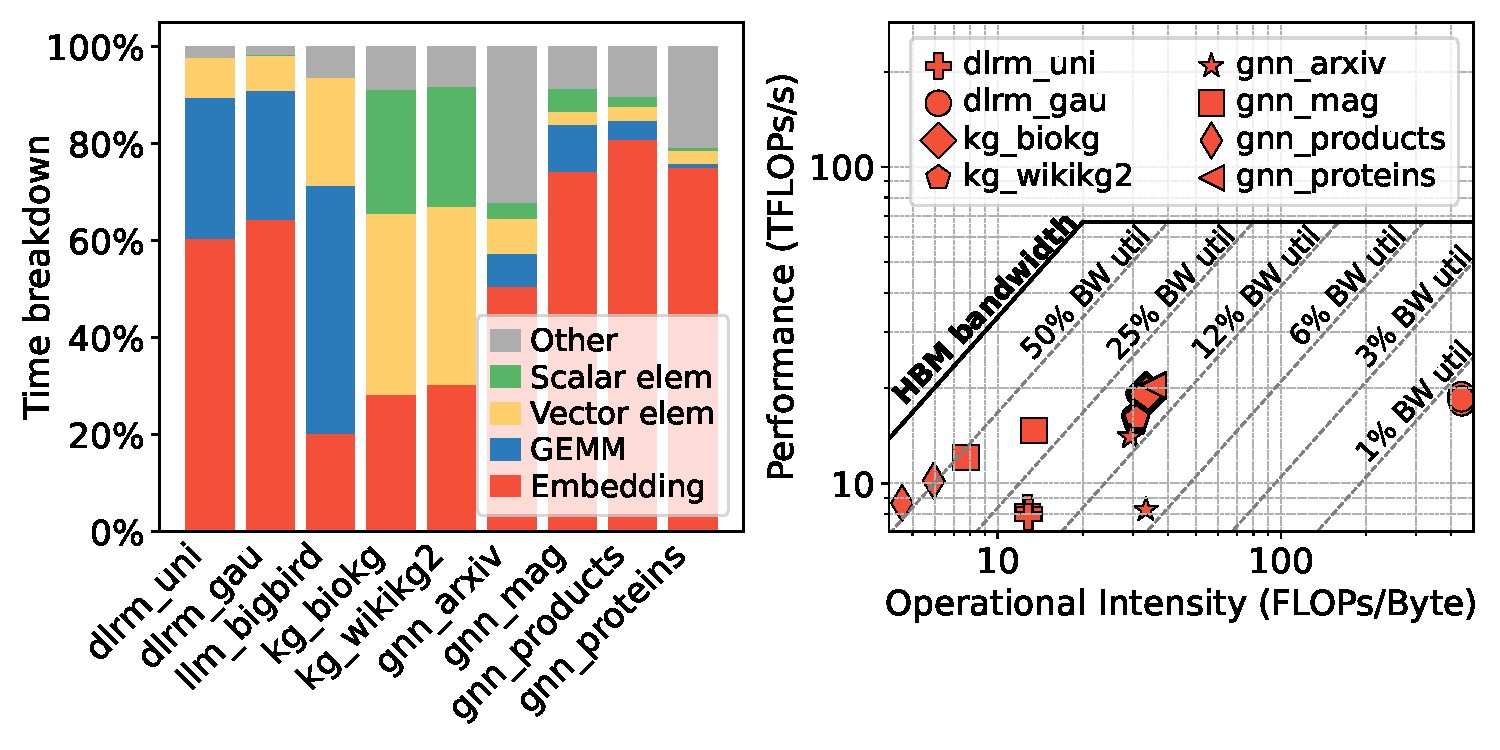
\includegraphics[width=.8\linewidth]{img_gpu_benchmark.pdf}
    \begin{subfigure}[b]{0.45\linewidth}
        \centering
        \vspace{-2em}
        \caption{Runtime breakdown}
        \label{fig:implications-embedding-gpu-runtime-breakdown}
    \end{subfigure}
    \begin{subfigure}[b]{0.45\linewidth}
        \centering
        \vspace{-2em}
        \caption{Roofline model}
        \label{fig:implications-embedding-gpu-roofline}
    \end{subfigure}
    \caption[Performance bottleneck of sparse ML models on GPU.]{Execution time breakdown and architectural utilization of sparse machine-learning models on an Nvidia H100 GPU~\cite{nvidia2024h100,nvidia2022hopper}. Subfigure~(a) reports the fraction of end-to-end kernel time spent in embedding lookup/aggregation, GEMM, vector elementwise operations, scalar elementwise operations, and other operations; each stacked bar is normalized to one workload. Subfigure~(b) shows a Roofline model for the embedding kernels only. The x-axis reports operational intensity, computed as embedding-kernel floating-point operations per byte transferred to and from GPU HBM during the measured kernel execution, and the y-axis reports achieved performance. Markers identify model/input pairs, and diagonal guide lines indicate fractions of peak HBM bandwidth utilization. In the end, embedding operations dominate the runtime of several sparse ML workloads, yet they do not map efficiently to GPU execution.}
    \label{fig:implications-embedding-gpu-performance}
\end{figure}

\Cref{fig:implications-embedding-gpu-runtime-breakdown} shows the runtime breakdown of these models on GPUs, which are the most widely used accelerators for machine learning applications. Overall, embedding operations consume roughly 60\%--80\% of cycles in GNNs and DLRMs. Because both GNNs and DLRMs pool the embedding vectors of neighboring entities, their embedding runtime scales roughly with the average number of neighbors. In other workloads, such as sparse LLMs and KGs, embedding operations still account for a sizable fraction of execution time, but GEMM and elementwise operations also contribute substantially.

\Cref{fig:implications-embedding-gpu-roofline} shows the Roofline model~\cite{williams2009roofline} for embedding operations. Overall, although these operations are critical, they achieve less than 30\% of peak compute utilization. As reported in \Cref{tab:embedding-workload-locality-characterization}, GNNs and KGs exhibit the lowest temporal locality and therefore the highest memory bandwidth utilization---yet even in these cases, bandwidth utilization remains below 55\%.

The operational intensity of these embedding kernels is higher than that of the sparse linear-algebra kernels in \Cref{fig:implications-scientific-roofline} because embedding operations generally exhibit higher temporal and spatial locality. Repeated embedding accesses improve cache reuse, while vector-valued lookups expose contiguous accesses within each embedding vector, reducing HBM traffic per operation.

Unlike typical machine learning operations (e.g., dense matrix multiplication), embedding operations look up embedding vectors from scattered memory locations and aggregate them with elementwise operations. GPUs, however, are designed for massively parallel and regular computation where (1)~memory accesses can be coalesced and (2)~there is sufficient computation to hide memory latency. In embedding workloads, (1)~embedding vectors are only hundreds of elements long, limiting coalescing opportunities, and (2)~elementwise operations do not provide enough computation to hide memory latency. Therefore, memory latency prevents GPUs from achieving high memory bandwidth utilization, compute utilization, and overall performance on these workloads~\cite{pellauer2023symphony}.

Combined with the high cost of GPUs and their limited memory capacity for storing large embedding tables, these inefficiencies make GPUs a poor target for embedding operations. Efficient support for these models must therefore be close to large memories and cannot rely solely on GPU-style coalescing or dense computation to hide lookup latency. To address this issue, several production systems offload embedding operations to CPUs while keeping dense neural network layers on GPUs~\cite{chen2023icde}, or execute the entire pipeline on CPUs~\cite{mudigere2022isca}. Although this solution is more cost-effective, commodity processors remain poorly optimized for the highly irregular memory accesses generated by embedding lookups, as demonstrated next.

\subsection{Embedding Performance on Off-the-Shelf CPUs} \label{sec:embedding-performance-cpus} %%%%%%%%%%%%%%%%%%%%%%%%%%%%%%%%%%%%%%%%%%

In this section, we show that embedding performance on commodity CPU cores is limited by the inability to sustain enough long-latency memory requests in flight. We demonstrate this with graph learning models, whose spatial and temporal locality span a broad range of the regimes observed across embedding workloads. This analysis shows how cache filtering, long-latency memory accesses, and core-side request tracking interact across inputs with different reuse patterns.

\begin{figure}
    \centering
    %\vspace{-1em}
    \begin{subfigure}[b]{0.49\linewidth} % 40% width
        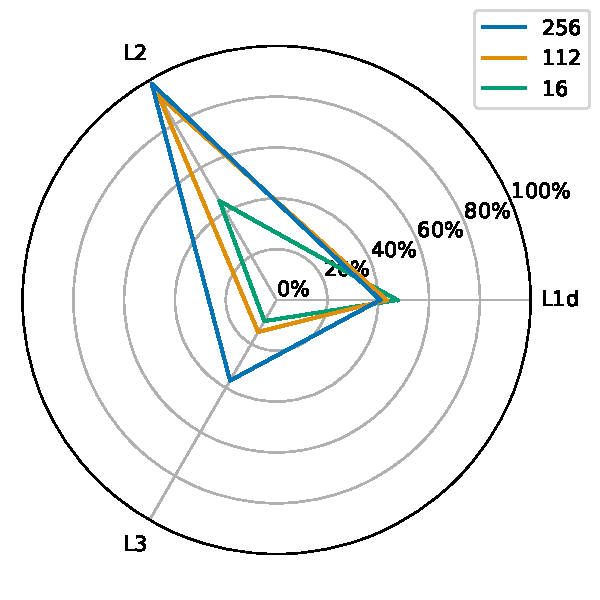
\includegraphics[width=\linewidth]{img_misses_proteins.pdf}
        \vspace{-2.2em}
        \caption{\texttt{proteins}}
        %\vspace{0.5em}
        \label{fig:miss-proteins}
    \end{subfigure}
    \begin{subfigure}[b]{0.49\linewidth} % 40% width
        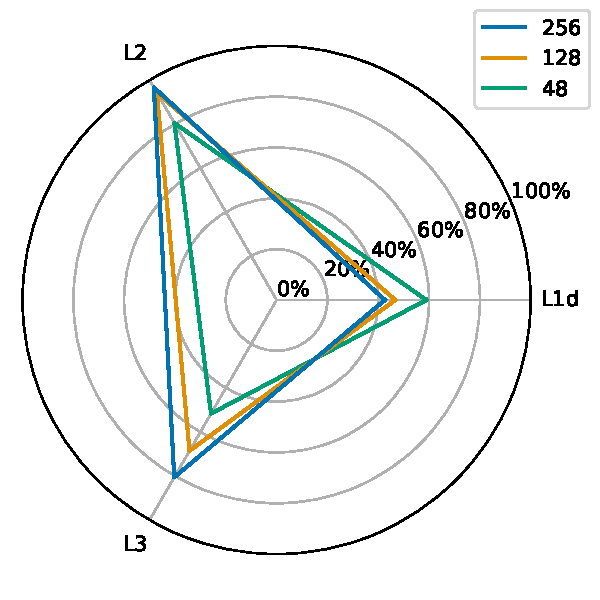
\includegraphics[width=\linewidth]{img_misses_arxiv.pdf}
        \vspace{-2.2em}
        \caption{\texttt{arxiv}}
        %\vspace{0.5em}
        \label{fig:miss-arxiv}
    \end{subfigure}
    \begin{subfigure}[b]{0.49\linewidth} % 40% width
        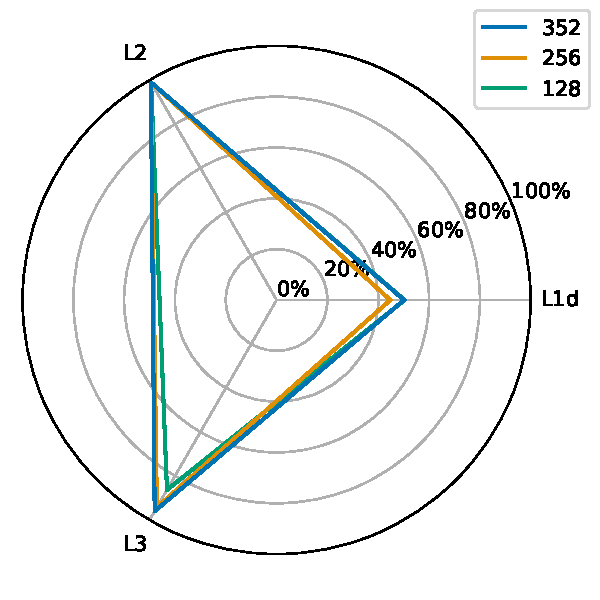
\includegraphics[width=\linewidth]{img_misses_mag.pdf}
        \vspace{-2.2em}
        \caption{\texttt{mag}}
        %\vspace{0.5em}
        \label{fig:miss-mag}
    \end{subfigure}
    \begin{subfigure}[b]{0.49\linewidth} % 40% width
        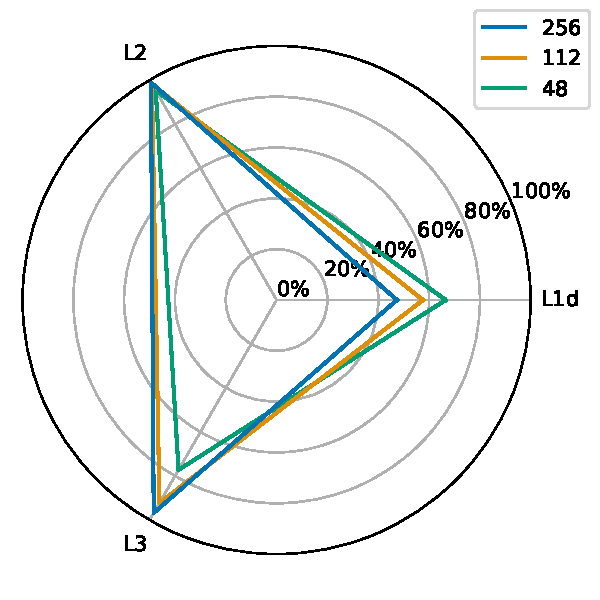
\includegraphics[width=\linewidth]{img_misses_products.pdf}
        \vspace{-2.2em}
        \caption{\texttt{products}}
        %\vspace{0.5em}
        \label{fig:miss-products}
    \end{subfigure}
    %\vspace{-1em}
    \caption[Cache miss rate for embedding lookups on CPU.]{Cache miss rate for GNN embedding lookups on the multicore CPU baseline. Each subfigure reports one input graph, and each line corresponds to one embedding-vector size. The radar axes report the L1D, L2, and L3 miss rates, computed as the percentage of vector requests that miss at each cache level. The high-locality graphs, \texttt{proteins} and \texttt{arxiv}, show substantially lower L3 miss rates because repeated accesses to nearby embedding vectors allow the LLC to filter many requests. In contrast, \texttt{mag} and \texttt{products} remain close to the outer rings for L2 and L3, indicating that most vector lookups continue to lower cache levels or HBM. Larger embedding vectors generally reduce L1D miss rates by exposing more spatial locality within each vector, but increase pressure on L2 and L3 because each cached vector occupies more capacity. Thus, L3 miss rates range from 38\% to 92\% across inputs and embedding sizes, showing that cache effectiveness depends strongly on graph locality and vector size.}
    \label{fig:misses}
\end{figure}


Overall, CPU cores are designed to access data primarily from local caches, which are populated by hardware prefetchers. However, these mechanisms are often ineffective for irregular embedding lookups, especially when reuse is low~\cite{gupta2020hpca}. \Cref{fig:implications-gnn-cache-misses} reports local miss rates for graphs from different domains, which exhibit distinct spatial and temporal locality characteristics. A local miss rate is the fraction of accesses to a given cache level that miss at that level. Overall, different graphs exhibit markedly different cache behaviors. More clustered graphs like \texttt{proteins} and \texttt{arxiv}, which reuse embedding vectors more frequently, achieve significantly better cache utilization. In contrast, sparser graphs like \texttt{mag} and \texttt{products} experience consistently high miss rates across the entire cache hierarchy. Furthermore, larger embedding vectors improve L1 cache behavior due to increased prefetching opportunities, but degrade performance at lower cache levels because of higher cache contention and eviction pressure. Overall, GNN layers experience L3 miss rates ranging from 38\% to 92\%, resulting in a substantial number of accesses to HBM memory.

\begin{figure}
    \centering
    %\vspace{-1em}
    \begin{subfigure}[b]{0.4\linewidth} % 40% width
        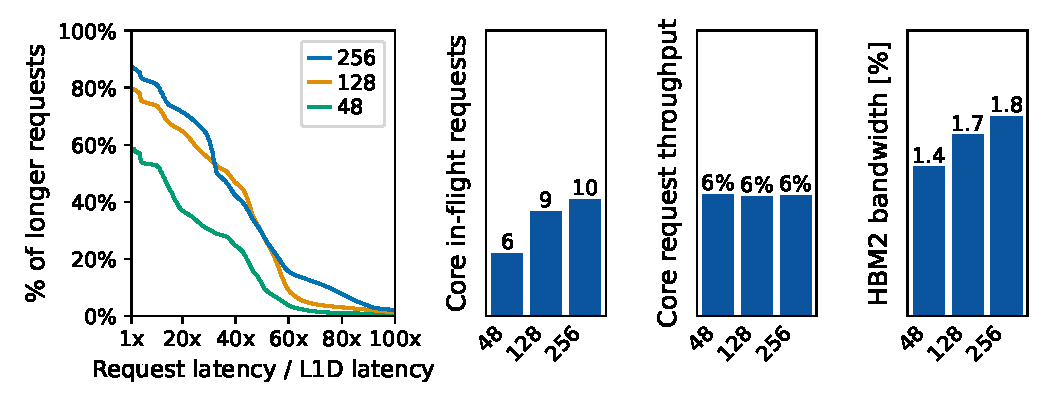
\includegraphics[width=\linewidth,trim=0 0 290 0,clip]{img_embedding_implications_arxiv.pdf}
        \vspace{-2em}
        \caption{\texttt{arxiv}}
        %\vspace{0.5em}
        %\label{fig:ltu-arxiv}
    \end{subfigure}
    \begin{subfigure}[b]{0.4\linewidth} % 40% width
        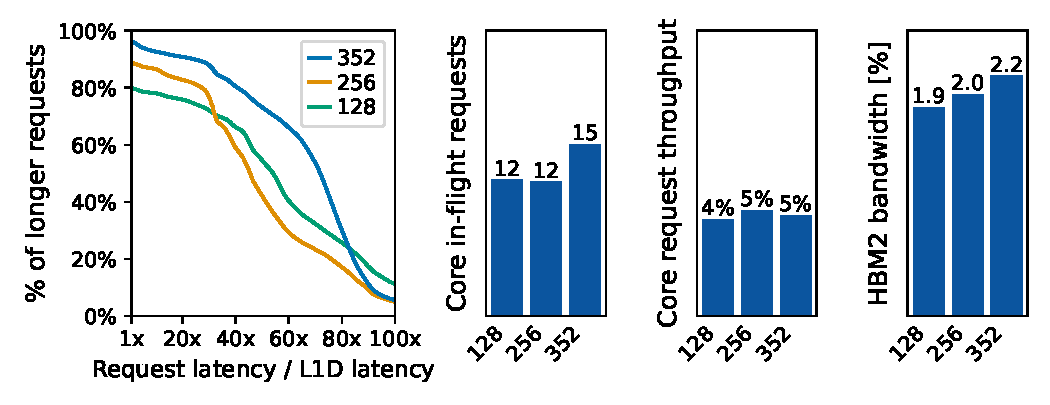
\includegraphics[width=\linewidth,trim=0 0 290 0,clip]{img_embedding_implications_mag.pdf}
        \vspace{-2em}
        \caption{\texttt{mag}}
        %\vspace{0.5em}
        %\label{fig:ltu-mag}
    \end{subfigure}
    \begin{subfigure}[b]{0.4\linewidth} % 40% width
        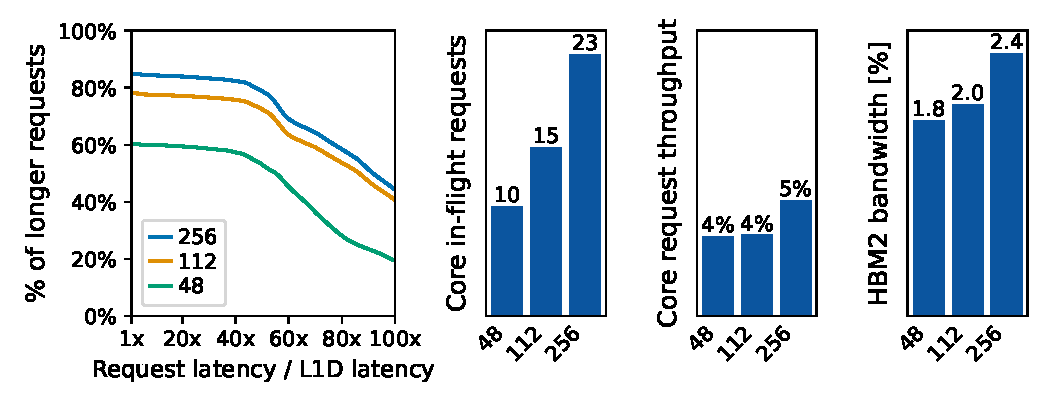
\includegraphics[width=\linewidth,trim=0 0 290 0,clip]{img_embedding_implications_products.pdf}
        \vspace{-2em}
        \caption{\texttt{products}}
        %\vspace{0.5em}
        %\label{fig:ltu-products}
    \end{subfigure}
    \begin{subfigure}[b]{0.4\linewidth} % 40% width
        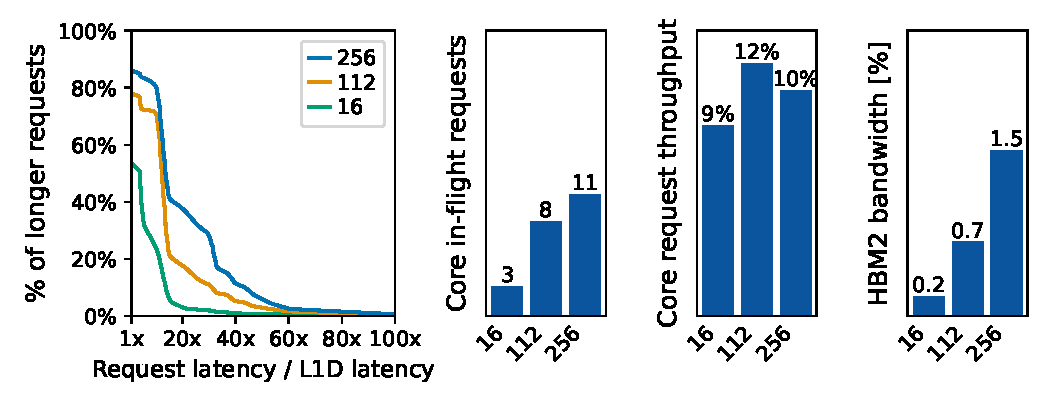
\includegraphics[width=\linewidth,trim=0 0 290 0,clip]{img_embedding_implications_proteins.pdf}
        \vspace{-2em}
        \caption{\texttt{proteins}}
        %\vspace{0.5em}
        %\label{fig:ltu-proteins}
    \end{subfigure}
    %\vspace{-2em}
    \caption[Load-to-use latency of embedding lookups on CPU.]{Load-to-use latency of GNN embedding lookups. The y-axis shows the percentage of requests longer than the corresponding value on the x-axis, which is computed as request latency relative to the latency of accessing the L1D cache. Overall, a large fraction of embedding lookups in GNN models take orders of magnitude longer than L1D accesses. For \texttt{products}---the dataset with the lowest locality---more than 74\% of memory requests (y-axis) are 10$\times$ longer than an L1D access (x-axis), and 40\% are more than 100$\times$ longer, as they need to reach HBM.}
    \label{fig:ltu-gnn}
\end{figure}

\begin{figure}
    \centering
    %\vspace{-1em}
    \begin{subfigure}[b]{0.45\linewidth} % 40% width
        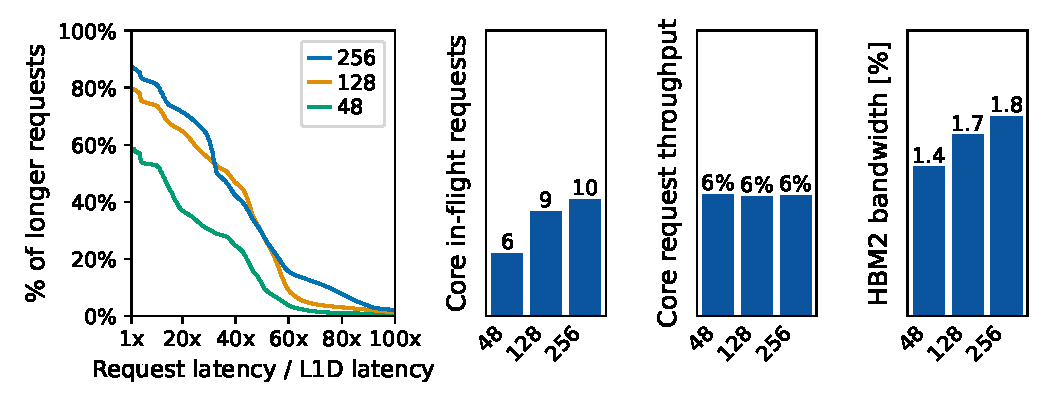
\includegraphics[width=\linewidth,trim=210 0 0 0,clip]{img_embedding_implications_arxiv.pdf}
        \vspace{-2em}
        \caption{\texttt{arxiv}}
        %\vspace{0.5em}
        %\label{fig:ltu-arxiv}
    \end{subfigure}
    \hspace{1cm} % <-- increase this to spread them
    \begin{subfigure}[b]{0.45\linewidth} % 40% width
        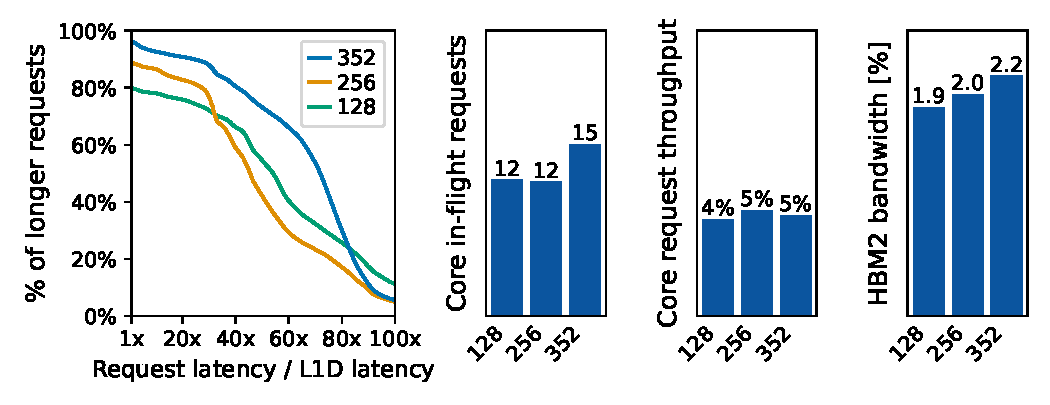
\includegraphics[width=\linewidth,trim=210 0 0 0,clip]{img_embedding_implications_mag.pdf}
        \vspace{-2em}
        \caption{\texttt{mag}}
        %\vspace{0.5em}
        %\label{fig:ltu-mag}
    \end{subfigure}
    \begin{subfigure}[b]{0.45\linewidth} % 40% width
        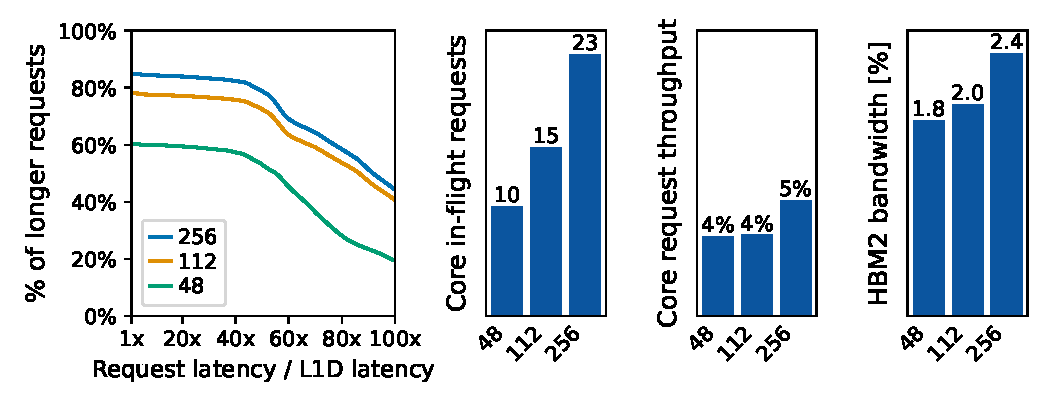
\includegraphics[width=\linewidth,trim=210 0 0 0,clip]{img_embedding_implications_products.pdf}
        \vspace{-2em}
        \caption{\texttt{products}}
        %\vspace{0.5em}
        %\label{fig:ltu-products}
    \end{subfigure}
    \hspace{1cm} % <-- increase this to spread them
    \begin{subfigure}[b]{0.45\linewidth} % 40% width
        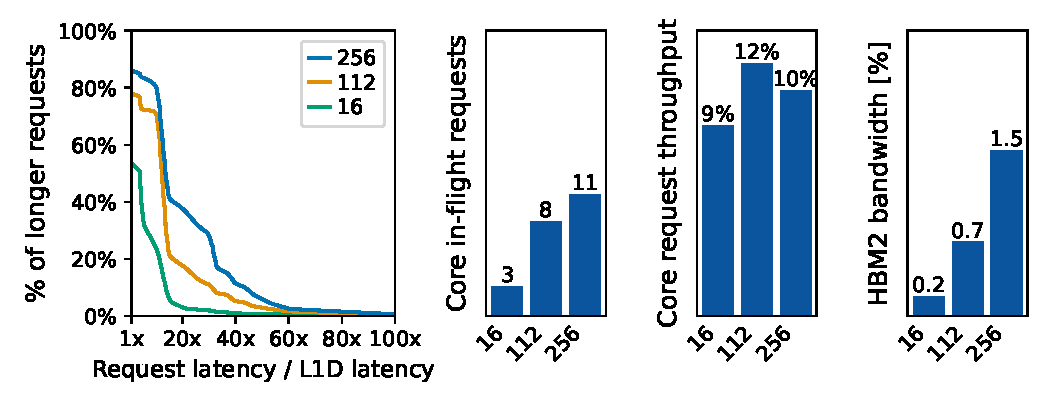
\includegraphics[width=\linewidth,trim=210 0 0 0,clip]{img_embedding_implications_proteins.pdf}
        \vspace{-2em}
        \caption{\texttt{proteins}}
        %\vspace{0.5em}
        %\label{fig:ltu-proteins}
    \end{subfigure}
    %\vspace{-2em}
    \caption[Architectural implications of embedding lookups on CPU.]{Architectural implications of long embedding lookups on an off-the-shelf CPU core. Bars correspond to different embedding sizes. The leftmost plot shows the average number of in-flight memory requests tracked by the core. The middle plot shows request throughput utilization, computed as actual request throughput relative to the peak throughput of one request per cycle. The rightmost plot shows memory bandwidth utilization. As shown in the leftmost plots, the higher the average latency, the higher the number of in-flight requests tracked by the core. However, because of their limited memory-level parallelism, CPU cores can only track a few requests before the whole pipeline stalls. As shown in the middle plots, due to these stalls, the core issues memory requests at a fraction of its peak throughput of one request per cycle. Even \texttt{proteins}---the dataset with the highest locality---only achieves up to 12\% throughput. As shown in the rightmost plots, this results in low HBM per-core utilization. Even a low-locality dataset like \texttt{products}---with the majority of accesses reaching HBM---utilizes up to 2.4\% bandwidth. Overall, off-the-shelf traditional cores are not optimized for long memory accesses.}
    \label{fig:embedding-implications}
\end{figure}


As a result, embedding lookups generate a high volume of long-latency memory requests~\cite{esmailidokht2024micro}. For instance, as shown in \Cref{fig:implications-gnn-load-latency}, up to 86\% of the memory requests in GNN embedding operations take more than $10\times$ the latency of an L1D cache access, and up to 36\% exceed $100\times$ that latency because they must reach HBM.

When a core issues a memory request, it must allocate entries in the reorder buffer, load--store queue, and miss-status handling registers at each cache level. The longer the memory access, the more entries are required to sustain multiple outstanding requests, a property generally known as memory-level parallelism. However, because these structures do not scale easily, traditional architectures provision just enough capacity to efficiently load data from local caches, not from HBM. As shown in \Cref{fig:implications-gnn-cpu-lookup-throughput}, off-the-shelf CPU cores achieve low request throughput across all inputs because long-latency embedding lookups require more memory-level parallelism than the core can sustainably provide~\cite{esmailidokht2024micro}, and because data-dependent traversal introduces additional control overhead. This results in low HBM utilization even for inputs whose requests mostly miss the caches and reach memory. Therefore, an efficient architecture for embedding operations must expose high memory-level parallelism without tying every in-flight vector lookup to scarce out-of-order core resources.

\subsection{Ideal Memory-Level Parallelism Requirements} \label{sec:ideal-mlp-requirements} %%%%%%%%%%%%%%%%%%%%%%%%%%%%%%%%%%

The previous section shows that commodity CPU cores cannot sustain enough irregular memory requests to execute embedding lookups efficiently. This section quantifies why simply scaling conventional cores is not a practical solution. We estimate the memory-level parallelism an ideal core would need to sustain peak embedding-lookup throughput: the model starts from a target request rate at the core, uses the reuse-distance CDF to determine which cache or memory level serves each request, and applies Little's rule to compute the number of outstanding requests required at the core and at each cache level. This gives a lower-bound estimate of the buffering and request-tracking resources that conventional cores would need to keep embedding lookups fully pipelined.

\begin{figure}
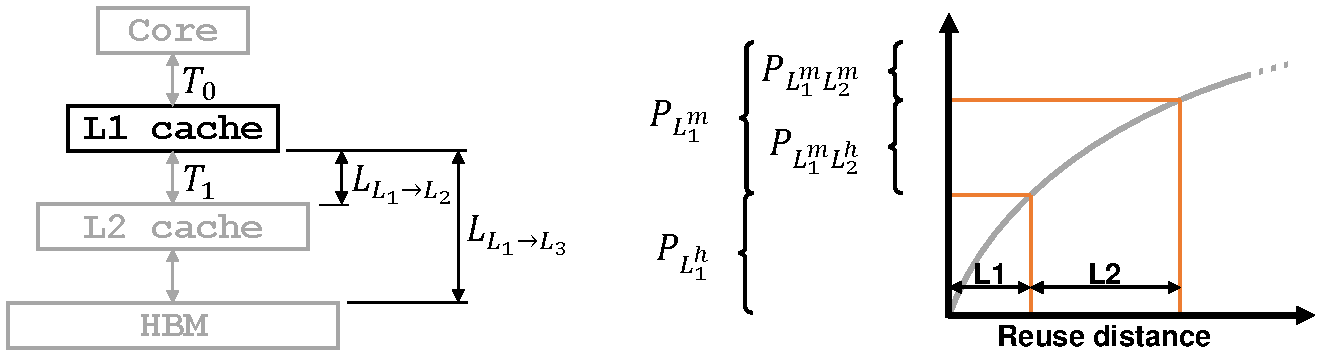
\includegraphics[width=1\linewidth]{img_abstraction_cdf.pdf}
    \begin{subfigure}[b]{0.48\linewidth}
        \centering
        \caption{System abstraction}
        \label{fig:implications-mlp-system-abstraction}
    \end{subfigure}
    \begin{subfigure}[b]{0.48\linewidth}
        \centering
        \caption{Reuse distance CDF}
        \label{fig:implications-mlp-reuse-cdf}
    \end{subfigure}
\caption[System abstraction for the analytical memory-level parallelism model.]{System abstraction used by the analytical memory-level parallelism model. Subfigure (a) models the core, cache hierarchy, and HBM as a sequence of levels with per-level latency and request throughput. Subfigure (b) shows how the reuse-distance CDF maps cache capacity, expressed as the number of embedding vectors that fit in each cache level, to hit and miss probabilities. This abstraction connects workload locality to the request rates and outstanding requests needed at each memory level.}
\label{fig:implications-mlp-analytical-model}
\end{figure}

\Cref{fig:implications-mlp-analytical-model} illustrates the system abstraction underlying our model. In \Cref{fig:implications-mlp-system-abstraction}, the system has $N$ logical levels, where $L_0$ is the core, $L_1 \ldots L_{N-2}$ are the caches, and $L_{N-1}$ is HBM. The latency to access level $L_b$ from level $L_a$ is $\lambda_{a \rightarrow b}$ clock cycles. For each level $L_x$, we define $T_x$ as the request throughput entering that level, measured in requests per cycle. Thus, $T_0$ is the request rate issued by the core, while $T_x$ for $x>0$ is the rate of requests that miss in previous levels and reach level $L_x$.

We compute the number of outstanding memory requests using Little's rule~\cite{little1961proof}, which states that, assuming the core issues memory requests at throughput $T_0$, the number of outstanding requests at each level is:
\begin{equation}
\label{eq:little-rule}
R_x = T_x \times \bar{\lambda}_x
\end{equation}
where both terms depend on the cache hit rate per level. Intuitively, the longer the memory requests or the higher the throughput, the higher the number of outstanding memory requests.

We define the cache hit or miss probability at levels $x$ and $y$ as $P_{L_x^{a_x} L_y^{a_y}}$, with $a_x, a_y \in \{\text{h}, \text{m}\} = \{\text{hit}, \text{miss}\}$. Moreover, we define the (conditional) probability of a hit or miss at level $x$ given a hit or miss at level $y$ as
\begin{equation}
P_{L_x^{a_x} | L_y^{a_y}} = P_{L_x^{a_x} L_y^{a_y}} / P_{L_y^{a_y}}.
\end{equation}
Hence, the \emph{output throughput} $T_x$ at level $x$ is 
\begin{equation}
T_x = T_{x-1} \times P_{L_x^{m} | L_1^{m} \ldots L_{x-1}^{m}} \;\text{cycle}^{-1},
\end{equation}
with $T_0$ the throughput at which the core issues memory requests.
Similarly, the \emph{average request latency} $\bar{\lambda}_x$ at level $x$ is
\begin{equation}
\bar{\lambda}_x =
\sum_{\ell = x+1}^{N-1}
\lambda_{x \rightarrow \ell} \times
P_{L_{x+1}^{m} \ldots L_{\ell-1}^{m} L_{\ell}^{h} | L_1^{m} \ldots L_x^{m}} \;\text{cycles}.
\end{equation}
We compute these probabilities from the spatial and temporal locality of the input model.

\begin{figure}
    \centering
    \begin{subfigure}[b]{0.4\linewidth}
        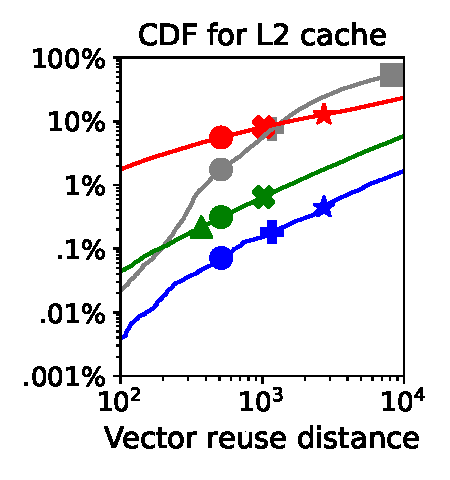
\includegraphics[width=.8\linewidth]{img_cdf2.pdf}
        \label{fig:implications-gnn-reuse-cdf-l2}
    \end{subfigure}
    \begin{subfigure}[b]{0.535\linewidth}
        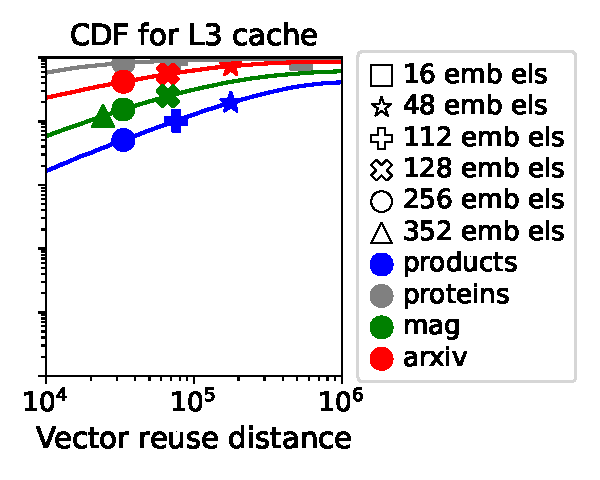
\includegraphics[width=.8\linewidth]{img_cdf3.pdf}
        \label{fig:implications-gnn-reuse-cdf-l3}
    \end{subfigure}
    \vspace{-1em}
\caption[Cumulative distribution functions of the reuse distance of the selected graphs.]{Reuse-distance CDFs for the GNN inputs in \Cref{tab:embedding-graph-inputs}, mapped to the L2 and L3 capacities of the CPU baseline in \Cref{tab:embedding-cpu-system-specs}. Both subfigures show the same reuse-distance CDFs, but use different x-axis ranges to make the L2 and L3 cache-capacity markers readable. The x-axis reports reuse distance in number of embedding-vector accesses, and the y-axis reports the fraction of accesses with reuse distance below that value; at each cache-capacity marker, this fraction approximates the probability that an access can be served by a cache of that capacity or smaller. Colors identify input graphs, while markers identify embedding-vector sizes, which determine how many vectors fit in L2 (left) or L3 (right). The expected fraction of accesses captured by the L2 capacity is low for most inputs: \texttt{products} ranges from 0.07\% to 0.46\%, \texttt{mag} from 0.22\% to 0.64\%, \texttt{arxiv} from 5.6\% to 13\%, and \texttt{proteins} from 1.7\% to 53\%. The L3 capacity substantially increases the expected captured fraction, but with large differences across graphs: \texttt{products} ranges from 5.1\% to 20\%, \texttt{mag} from 12\% to 25\%, \texttt{arxiv} from 42\% to 76\%, and \texttt{proteins} from 82\% to 96\%. Together with the measured miss rates in \Cref{fig:implications-gnn-cache-misses}, these trends suggest that reuse-distance CDFs can predict cache behavior.}
\label{fig:implications-gnn-reuse-cdfs}
\end{figure}

As discussed in \Cref{sec:embedding-workload-characterization}, we model spatial locality via the embedding vector size, and temporal locality via the CDF of the reuse distance~\cite{ding2003pldi}. Recall that the reuse distance is the number of other embedding vectors accessed before a vector is accessed again. If a cache can hold $x$ vectors, an access with reuse distance greater than $x$ will likely result in eviction. Hence, we can model the hit or miss probability of a given cache as the fraction of accesses with reuse distance smaller or greater than $x$. We model such probabilities by first constructing a histogram of all reuse distances, which we then integrate and normalize to obtain the CDF. Thus, $CDF(x)$ approximates the hit probability of that cache, and \Cref{fig:implications-mlp-reuse-cdf} shows how to derive the above probabilities starting from the CDF. \Cref{fig:implications-gnn-reuse-cdfs} characterizes the graphs in \Cref{tab:embedding-graph-inputs}; the CDF trends match the measured cache behavior in \Cref{fig:implications-gnn-cache-misses}, suggesting that reuse-distance CDFs are a promising predictor of cache performance. We now validate this connection directly against gem5.

\begin{figure}
    \centering
    \begin{subfigure}[b]{0.32\linewidth}
        \centering
        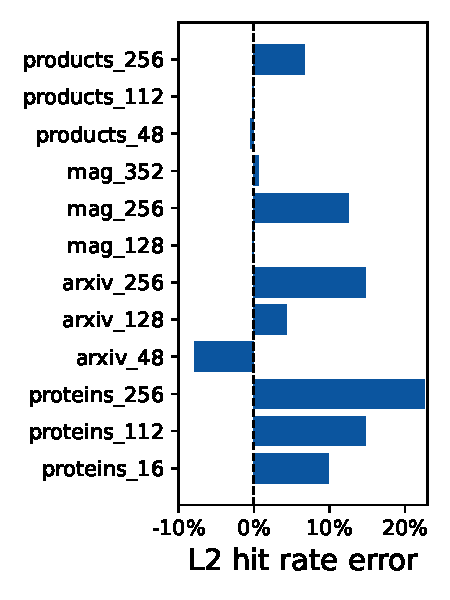
\includegraphics[width=\linewidth]{img_cpu_l2_hit_prediction_accuracy.pdf}
        \vspace{-1.5em}
        \caption{}
        \label{fig:implications-mlp-l2-hit-error}
    \end{subfigure}
    \begin{subfigure}[b]{0.44\linewidth}
        \centering
        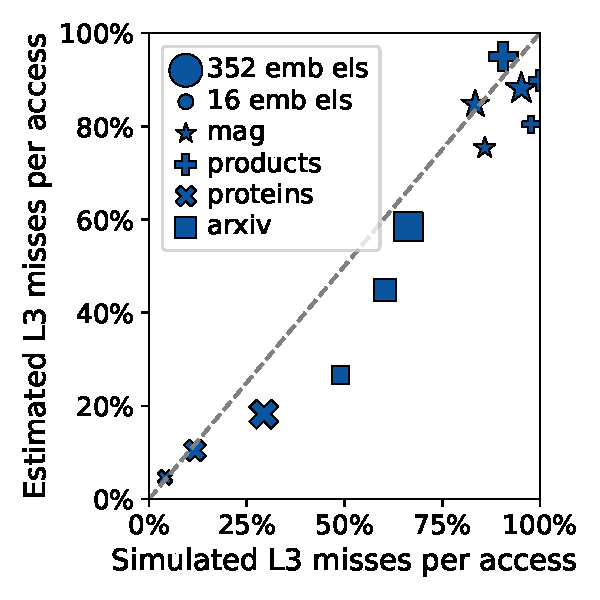
\includegraphics[width=\linewidth]{img_cpu_l3_hit_prediction_accuracy.pdf}
        \vspace{-1.5em}
        \caption{}
        \label{fig:implications-mlp-l3-miss-error}
    \end{subfigure}
    \begin{subfigure}[b]{0.22\linewidth}
        \centering
        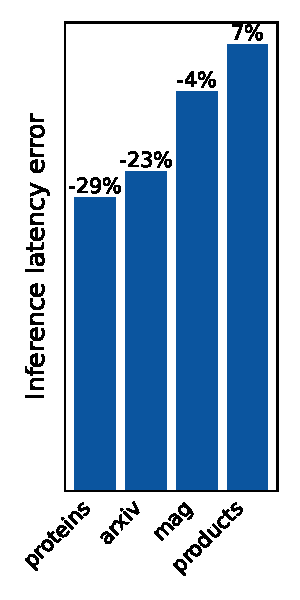
\includegraphics[width=\linewidth]{img_latency_error_bars.pdf}
        \vspace{-1.5em}
        \caption{}
        \label{fig:implications-mlp-cycle-error}
    \end{subfigure}
\caption[Accuracy of our analytical model compared to gem5.]{Accuracy of the analytical model compared with gem5, using the GNN inputs in \Cref{tab:embedding-graph-inputs} on the CPU baseline in \Cref{tab:embedding-cpu-system-specs}. Subfigure~(a) reports L2 hit-rate prediction error; positive values indicate that the model overestimates the gem5 hit rate, and negative values indicate underestimation. Across layers, L2 error ranges from -8 to +23 percentage points, with an average absolute error of roughly 8 percentage points. Subfigure~(b) compares simulated and estimated L3 misses per access. The dashed diagonal indicates perfect agreement, marker shape identifies the input graph, and marker size identifies the embedding-vector size. The model preserves the main trend: low-miss cases remain low, high-miss cases remain high, and points with more than 80\% simulated L3 misses stay close to the diagonal, although the model underestimates some midrange cases. Subfigure~(c) reports end-to-end execution-cycle error per input graph; errors range from -29\% for \texttt{proteins} to +7\% for \texttt{products}, with roughly 16\% average absolute error. Thus, the CDF-based model is accurate enough to capture cache behavior and execution-cycle trends for the memory-level-parallelism analysis, providing reasonable accuracy for an analytical model intended to predict trends rather than exact cycle counts~\cite{cabezas2014iisw}.}
\label{fig:implications-mlp-model-validation}
\end{figure}

\Cref{fig:implications-mlp-l2-hit-error} shows that our model estimates L2 accesses within 23\% error, whereas \Cref{fig:implications-mlp-l3-miss-error} shows similar behavior for L3 accesses, especially for high miss rates, which are the most relevant for our analysis. We now use these cache-access probabilities to estimate the end-to-end execution cost of embedding inference. At a high level, the model first computes the execution cycles and memory-level parallelism required by ideal execution, then compares these requirements with the maximum throughput and request-tracking capacity of each memory-system level, and finally rescales the ideal cycle count according to the most restrictive resource. The model represents ideal execution with the throughput $T^i_\ell$ and number of outstanding requests $R^i_\ell$ required at each memory level $\ell$, where the superscript $i$ indicates \emph{ideal}. We start by computing the \emph{ideal execution cycles} when running at full core throughput (one load per cycle per port):
\begin{equation}
C^i = \left\lceil \frac{\text{numLookups} \times \text{numLoadsPerLookup}}{\text{numReadPorts}} \right\rceil
\end{equation}
where \texttt{numLookups} is the number of loaded embedding vectors, \texttt{numLoadsPerLookup} is the number of vector loads required to fetch an embedding vector, and \texttt{numReadPorts} is the number of read ports out of the core. Given a system where each component at level $\ell$ has:
\begin{itemize}
    \item \emph{max throughput} $T^m_\ell$ (bounded by its ports and frequency),
    \item \emph{max number of requests} $R^m_\ell$ (bounded by MSHRs),
\end{itemize}
where the superscript $m$ indicates \emph{maximum}. Rather than composing these limits across memory levels, we use a bottleneck model: each resource determines the fraction of ideal execution it can sustain, and the most restrictive resource sets the overall scaling factor. We define the fraction of ideal execution that each component at level $\ell$ can sustain as:
\begin{equation}
S^{t}_\ell = \min \left( 1, \frac{T^m_\ell}{T^i_\ell} \right)
\end{equation}
for throughput, and
\begin{equation}
S^{r}_\ell = \min \left( 1, \frac{R^m_\ell}{R^i_\ell} \right)
\end{equation}
for request tracking capacity. These scaling factors are 1 when the corresponding resource can sustain ideal execution and smaller than 1 when it becomes a bottleneck. We then compute the limiting scaling factor $S$ as:
\begin{equation}
S = \min \left( \min_\ell S^{t}_\ell, \min_\ell S^{r}_\ell \right).
\end{equation}
Finally, we compute the \emph{estimated execution cycles} $C^e$ by rescaling the ideal execution cycles $C^i$ according to this bottleneck scaling factor:
\begin{equation}
C^e = \frac{C^i}{S}.
\end{equation}
Execution time is then obtained by dividing these cycle counts by the core frequency. \Cref{fig:implications-mlp-cycle-error} validates this estimate by showing that the model estimates the end-to-end execution cycles of the entire embedding operation within 29\% error, which is reasonable for an analytical model intended to predict trends rather than exact cycle counts~\cite{cabezas2014iisw}. This level of accuracy suggests that the locality and memory-system parameters captured by the model are sufficient to explain the dominant performance behavior of these workloads.

\begin{figure}
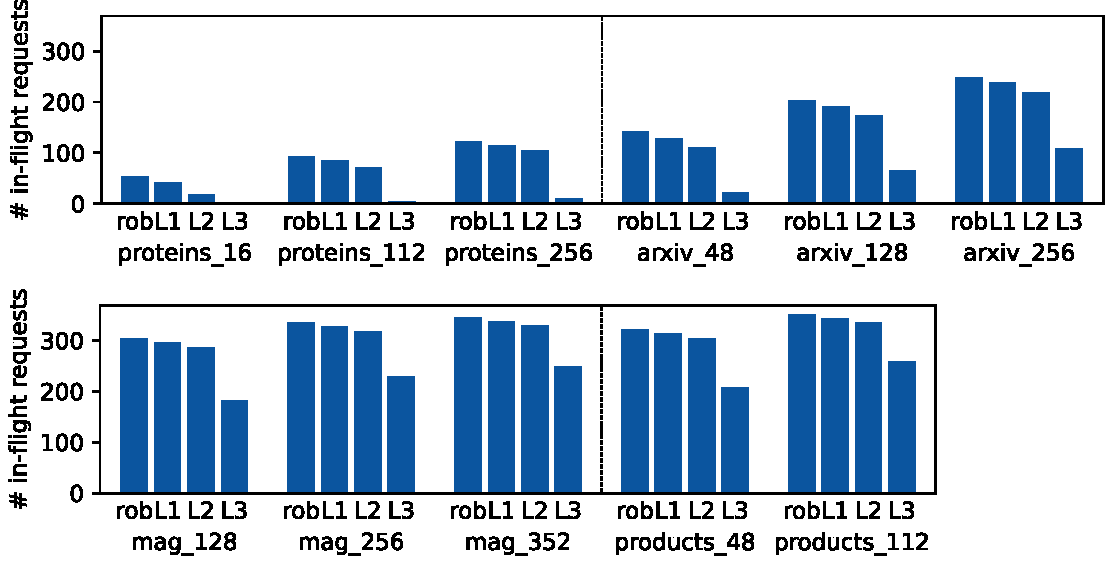
\includegraphics[width=1\linewidth]{img_max_mlp_stacked.pdf} % L B R T
\vspace{-2em}
\caption[Ideal memory-level parallelism on CPU.]{Outstanding requests required to sustain ideal GNN embedding-lookup throughput on the CPU baseline in \Cref{tab:embedding-cpu-system-specs}. These values are lower-bound requirements computed with the analytical model described in this section (\Cref{eq:little-rule}), assuming an ideal core-side request rate of one embedding-vector load per cycle and accounting for the cache hit and miss probabilities derived from the reuse-distance CDFs. Each group of bars corresponds to one evaluated layer, identified by input graph and embedding-vector size. Within each group, the \texttt{rob} bar reports the number of requests that must remain in flight at the core, while the L1, L2, and L3 bars report the corresponding MSHR demand at each cache level after cache filtering. The required memory-level parallelism grows with lower temporal locality and larger vectors: \texttt{proteins\_16} requires only 55 core-level requests and roughly one L3 request, whereas \texttt{products\_112} reaches 368 core-level requests and 270 L3 requests. Across all layers, the average demand is about 241, 230, 216, and 127 requests at the core, L1, L2, and L3 levels, respectively. Thus, sustaining ideal embedding throughput would require far more in-flight request tracking than conventional out-of-order cores and cache MSHR structures are designed to provide.}
\label{fig:implications-gnn-ideal-mlp}
\end{figure}

We now leverage \Cref{eq:little-rule}, Little's rule, to estimate the number of outstanding requests per core required to run at peak throughput (one load per cycle per port). This ideal request rate is not intended to model achieved execution on a conventional core; rather, it asks how much memory-level parallelism the memory system would need to sustain if the core-side pipeline were not the bottleneck. \Cref{fig:implications-gnn-ideal-mlp} shows that this would require up to 368 outstanding requests per core, 241 on average. In the next section, we demonstrate that traditional cores cannot achieve such memory-level parallelism.


\subsection{The Cost of Scaling Memory-Level Parallelism} \label{sec:cost-of-scaling-mlp} %%%%%%%%%%%%%%%%%%%%%%%%%%%%%%%%%%%%%%%%%%

\begin{figure}
    \centering
    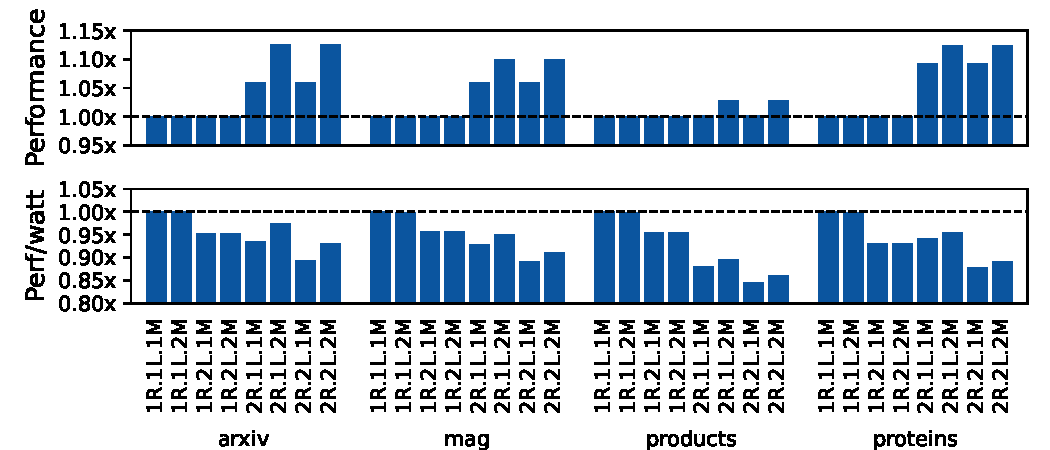
\includegraphics[width=\linewidth]{img_dse_cpu.pdf}
    \vspace{-1em}
    \caption[The cost of scaling memory-level parallelism on CPU.]{Cost of scaling memory-level parallelism in the CPU baseline from \Cref{tab:embedding-cpu-system-specs} for GNN embedding operations. The top plot reports performance normalized to the baseline core, and the bottom plot reports normalized performance per watt; dashed horizontal lines mark the baseline value of 1$\times$. Groups correspond to input graphs, and bars within each group correspond to different resource-scaling configurations. In the configuration names, \texttt{R} denotes reorder buffer and register-file capacity, \texttt{L} denotes load--store queue capacity, and \texttt{M} denotes L1D MSHR capacity; \texttt{1R.1L.1M} is the baseline core, while \texttt{2R.2L.2M} doubles all three resources. Scaling only \texttt{L} or \texttt{M} provides essentially no performance improvement, while scaling \texttt{R} provides most of the gains. Even the fully scaled core improves performance by only 1.03$\times$--1.13$\times$ across inputs, but reduces performance per watt to 0.86$\times$--0.93$\times$ because power increases by roughly 20\%--26\%. Thus, scaling conventional core structures is an inefficient way to provide the memory-level parallelism required by embedding lookups.}
    \label{fig:implications-cpu-mlp-scaling-cost}
\end{figure}

Increasing the memory-level parallelism of a CPU core to track more in-flight requests requires scaling up the reorder buffer, load--store queue, and miss-status handling registers~\cite{sgherzi2024jpdc}. However, these resources scale inefficiently. As shown in \Cref{fig:implications-cpu-mlp-scaling-cost}, for datasets with high reuse, doubling them improves performance by only 12\% while increasing power consumption by 25\%, whereas for datasets with low reuse, it improves performance by 3\% while increasing power consumption by 18\%. In addition to degrading performance per watt, scaling up these resources introduces timing-closure challenges~\cite{siracusa2022tc}, which would require lowering the core frequency and, consequently, overall performance.

Another option is to scale out the number of cores or hardware threads. This can increase the number of outstanding memory requests, but it does not remove the underlying inefficiency: the system must still provision enough shared MSHRs, interconnect bandwidth, and memory-system queues to track those requests, while also replicating core structures that provide little benefit for memory-dominated embedding lookups. As shown in \Cref{fig:implications-gnn-cpu-lookup-throughput}, saturating a single HBM stack would require 43--72 traditional CPU cores, depending on input reuse. Thus, while scale-out can expose memory-level parallelism, it does so by scaling general-purpose execution resources along with the memory-request machinery. These results point to the same design principle as the scientific workloads: sparse accesses should be decoupled from the compute pipeline so that memory-level parallelism can scale without proportionally scaling expensive core structures.

\section{Summary} \label{sec:architectural-implications-summary}

In this chapter, we have demonstrated that traditional architectures that tightly couple control flow, memory access, and computation are fundamentally inadequate for sparse tensor algebra workloads. Scientific kernels show that traversal, scan-and-lookup operations, and coordinate merging leave both compute units and memory bandwidth underutilized. Machine learning embedding operations confirm this bottleneck across a wide range of spatial and temporal locality regimes. Scaling conventional cores up or out does not provide this memory-level parallelism efficiently. In the next chapter, we demonstrate how decoupling sparse traversal, merging, and marshaling from vector computation can overcome these limitations and substantially improve performance and efficiency.
